\documentclass[11pt]{scrartcl}
\usepackage[pretty,polish]{mystd}
\title{Algebra}
\author{Michał Dobranowski}
\date{semestr zimowy 2022 \\ v0.14}

\begin{document}
    \maketitle
    \begin{abstract}
        Poniższy skrypt zawiera materiał obejmujący wykłady z Algebry prowadzone przez dr hab. Jakuba Przybyło na I semestrze Informatyki na AGH oraz tematy, które uznałem za warte uwagi podczas własnych studiów nad tematem.
    \end{abstract}
    \tableofcontents
    \eject

    \section{Liczy zespolone}
    \begin{definition}
    Liczba zespolona $z$ to uporządkowana para liczb rzeczywistych. Pierwszy element tej pary to \vocab{część rzeczywista}, oznaczana symbolem $\Re(z)$, a drugi to \vocab{część urojona}, oznaczana symbolem $\Im(z)$. Zbiór liczb zespolonych oznaczamy przez $\CC$.
\end{definition}

Liczby zespolone można reprezentować w kilku postaciach, jedna z nich to \vocab{postać algebraiczna}. Używając jej, liczba $z = (x, y)$ jest zapisywana jako
$$ z = x + iy, $$
gdzie $i$ nazywamy \vocab{jednostką urojoną}, która spełnia
$$ i^2 = -1. $$

Niech $z_1 = x_1 + iy_1$ oraz $z_2 = x_2 + iy_2$. Określamy:
\begin{itemize}
    \item dodawanie $z_1 + z_2 = x_1 + x_2 + i(y_1 + y_2)$,
    \item mnożenie $\begin{aligned}[t] z_1z_2 &= x_1x_2 + ix_1y_2 + ix_2y_1 + i^2y_1y_2 \\ &= x_1x_2 - y_1y_2 + i(x_1y_2 + x_2y_1).\end{aligned}$
\end{itemize}

\begin{corollary}
    Dodawanie i mnożenie liczb zespolonych jest przemienne i łączne. Mnożenie jest rozdzielne względem dodawania.
\end{corollary}

\begin{definition}
    Sprzężenie liczby zespolonej $z = x + iy$ to liczba $\ol{z} = x - iy$.
\end{definition}

\begin{definition}
    \label{d:magnitude}
    Moduł liczby zespolonej $z = x + iy$ to liczba $|z| = \sqrt{x^2 + y^2}$.
\end{definition}

Zachodzi pewna własność, wynikająca ze wzoru skróconego mnożenia:
$$ z\ol{z} = (x + iy)(x - iy) = x^2 - i^2y^2 = x^2 + y^2 $$
\begin{equation}
    z\ol{z} = |z|^2
\end{equation}

Powyższa liczba jest liczbą rzeczywistą, więc znaleźliśmy prosty sposób na dzielenie liczb zespolonych przez siebie, mnożąc licznik i mianownik przez sprzężenie mianownika. Na przykład:
$$ \frac{1 + 2i}{-1 - i} = \frac{(1 + 2i)(-1 + i)}{(-1 - i)(-1 + i)} = \frac{-3 -i}{2} = \frac{-3}{2} - \frac{i}{2}. $$

\begin{lemma}
    Oprócz $z\ol{z} = |z|^2$, zachodzą również równości:
    \begin{itemize}
        \item $|\ol{z}| = |z|$
        \item $\ol{z_1 + z_2} = \ol{z_1} + \ol{z_2}$
        \item $\ol{z_1z_2} = \ol{z_1}\cdot\ol{z_2}$
        \item $|z_1z_2| = |z_1||z_2|$
    \end{itemize}
\end{lemma}
Ich dowody można w łatwy sposób przeprowadzić z definicji poszczególnych działań.

\subsection{Interpretacja geometryczna liczb zespolonych}
Liczby zespolone można interpretować jako punkty na \vocab{płaszczyźnie zespolonej}. Dla przykładu liczba $z = 3 + 2i$.

\begin{center}
    \begin{tikzpicture}
        \tkzInit[xmin=-.7, xmax=3.7, ymin=-.7, ymax=2.7]
        \tkzDefPoints{0/0/O,3/2/z}
        \tkzGrid
        \tkzDrawX[label=$\Re$,thick] \tkzDrawY[label=$\Im$,thick]
        \tkzDrawSegments(O,z)
        \tkzDrawPoints(z)
        \tkzLabelPoints[above right](z)
    \end{tikzpicture}
\end{center}

\begin{fact}
    Moduł liczby zespolonej $z$ to długość wektora wodzącego tej liczby na płaszczyźnie zespolonej.
\end{fact}
\begin{proof}
    Wynika to z twierdzenia Pitagorasa oraz definicji modułu (\ref{d:magnitude}).
\end{proof}

Możemy wyprowadzić \vocab{postać trygonometryczną} liczby zespolonej, która będzie operować na długości wektora wodzącego oraz kącie skierowanym. Mamy więc
$$ z = |z|(\cos\varphi + i\sin\varphi) $$
gdzie $\varphi$ to miara kąta skierowanego między wektorem wodzącym liczby zespolonej $z$ a~osią liczb rzeczywistych. Ten kąt nazywany jest \vocab{argumentem} i oznaczany przez $\Arg(z)$. Argument nie jest określony jednoznacznie -- dowolne dwa argumenty jednej liczby różnią się o wielokrotność $2\pi$. Jeśli argument jest w przedziale $[0, 2\pi)$, to mówimy, że jest to \vocab{argument główny} liczby $z$ i oznaczamy $\arg(z)$.

Za pomocą podstawowej trygonometrii możemy łatwo zamieniać postać algebraiczną i trygonometryczną między sobą.

\begin{center}
    \begin{tikzpicture}
        \tkzInit[xmin=-.7, xmax=3.7, ymin=-.7, ymax=2.7]
        \tkzDefPoints{0/0/O,1/0/A,3/2/z}
        \tkzDefPointBy[projection=onto O--A](z) \tkzGetPoint{z'}
        \tkzGrid
        \tkzDrawX[label=$\Re$,thick] \tkzDrawY[label=$\Im$,thick]
        \tkzDrawSegment[dim={$|z|$,2mm,}, dim style/.style={sloped,dashed}](O,z)
        \tkzDrawSegment[dim={$|z|\cos\varphi$,-2mm,}, dim style/.style={sloped,dashed}](O,z')
        \tkzDrawSegment[dim={$|z|\sin\varphi$,2mm,}, dim style/.style={sloped,dashed}](z,z')
        \tkzMarkAngle[size=1.1](z',O,z)
        \tkzLabelAngle[pos=.8](z',O,z){$\varphi$}
        \tkzDrawPoints(z)
        \tkzLabelPoints[above right](z)
    \end{tikzpicture}
\end{center}

\begin{equation}
    \Re{z} = |z|\cos\varphi, \hspace{2em} \Im{z} = |z|\sin\varphi
\end{equation}

Na potrzeby dalszych rozważań przyjmujemy, że $\arg(0) = 0$.

\begin{fact}
    Odległość między liczbami $z_1$ i $z_2$ na płaszczyźnie zespolonej wynosi $|z_1 - z_2|$.
\end{fact}

\begin{lemma}
    Zachodzą następujące nierówności:
    \begin{itemize}
        \item $|z_1 + z_2| \leq |z_1| + |z_2|$
        \item $||z_1| - |z_2|| \leq |z_1 - z_2|$
    \end{itemize}
\end{lemma}

Możemy łatwo mnożyć dwie liczby zespolone w postaci trygonometrycznej przez siebie za pomocą poniższego wzoru.
\begin{equation}
    \label{eq:complex_prod}
    \begin{aligned}
        z_1 \cdot z_2 &= |z_1|(\cos\varphi_1 + i\sin\varphi_1)|z_2|(\cos\varphi_2 + i\sin\varphi_2) \\
                      &= |z_1||z_2|(\cos\varphi_1\cos\varphi_2 - \sin\varphi_1\sin\varphi_2 + i(\cos\varphi_1\sin\varphi_2 + \sin\varphi_1\cos\varphi_2)) \\
                      &= |z_1||z_2|(\cos(\varphi_1 + \varphi_2) + i\sin(\varphi_1 + \varphi_2))
    \end{aligned}
\end{equation}

Stosując wzór \ref{eq:complex_prod} $n$ razy otrzymujemy dowód następującego twierdzenia.

\begin{theorem}[wzór de Moivre'a]
    \label{t:demoivre}
    Dla $z = |z|(\cos\varphi + i\sin\varphi)$ oraz $n \in \ZZ$ zachodzi równość
    $$ z^n = |z|^n(\cos n\varphi + i\sin n\varphi) $$
\end{theorem}

Wzór de Moivre'a zapewnia prosty sposób na potęgowanie liczb zespolonych. Dlatego, mając za zadanie obliczyć
$$ (-2\sqrt{3} - 2i)^{16} $$
najłatwiej będzie zmienić postać liczby do postaci trygonometrycznej, a następnie skorzystać ze wzoru de Moivre'a.

\begin{definition}[pierwiastek liczby zespolonej]
    Jeśli $z$ jest liczbą zespoloną, to $\sqrt[n]{z}$ jest zbiorem wszystkich takich $w \in \CC$, że $w^n = z$.
\end{definition}

Korzystając ze wzoru de Moivre'a (twierdzenie \ref{t:demoivre}), łatwo wyprowadzić wzór
\begin{equation}
    \label{eq:complex_root}
    \sqrt[n]{z} = \sqrt[n]{|z|}\left(\cos\frac{\varphi + 2k\pi}{n} + i\sin\frac{\varphi + 2k\pi}{n}\right), k \in \ZZ
\end{equation}

\begin{fact}
    Pierwiastków $n$-tego stopnia z $z \neq 0$ jest dokładnie $n$ i leżą one w równych odstępach na okręgu o środku w $0$ i promieniu $\sqrt[n]{|z|}$.
\end{fact}
\begin{proof}
    Dla $k \in \{0, 1, \ldots, n-1\}$ liczba z równości \ref{eq:complex_root} będzie przyjmować różne wartości (wynika to z okresowości funkcji trygonometrycznych). Liczby te będą na wspomnianym okręgu (to wynika wprost z postaci trygonometrycznej), a ich argumenty główne różnić będzie wielokrotność $\frac{2\pi}{n}$.
\end{proof}

\subsection{Postać wykładnicza}
Postać $z = |z|e^{i\varphi}$ liczby zespolonej będziemy nazywać \vocab{postacią wykładniczą} tej liczby.

\begin{theorem}[wzór Eulera]
    Dla każdego $\varphi \in \RR$ zachodzi
    $$ e^{i\varphi} = \cos\varphi + i\sin\varphi. $$
\end{theorem}
\begin{proof}
    Standardowo dowodzi się wzoru Eulera za pomocą szeregów Taylora. Pokażemy inny, mniej oczywisty, ale bardziej elementarny dowód.

    Niech $f(\varphi) = e^{-i\varphi}\left(\cos\varphi + i\sin\varphi\right)$. Zróżniczkujmy:
    \begin{align*}
        f'(\varphi) &= -ie^{-i\varphi}\left(\cos\varphi + i\sin\varphi\right) + e^{-i\varphi}\left(-\sin\varphi + i\cos\varphi\right) = \\
        &= e^{-i\varphi}\left(-i\cos\varphi + i\cos\varphi + \sin\varphi - \sin\varphi\right) = 0.
    \end{align*}
    Z tego wynika, że funkcja $f$ jest stała, więc
    \[ f(\varphi) \equiv f(0) = 1, \]
    \[ \therefore e^{i\varphi} = \cos\varphi + i\sin\varphi. \]
\end{proof}

    \section{Relacje}
    \begin{definition}
    Relacja to trójka $\sR = (X, \gr\sR, Y)$, gdzie $X$ i $Y$ są zbiorami, a $\gr \sR \subset X \times Y$.
\end{definition}

Zbiór $X$ nazywamy \vocab{naddziedziną}, $Y$ \vocab{zapasem}, $\gr \sR$ to \vocab{wykres} relacji. Piszemy, że $x \sR y$, jesli $(x, y) \in \gr\sR$. \vocab{Dziedzina} relacji $\sR$ to zbiór
$$ D_\sR = \{x \in X : \exists y \in Y : x \sR y\}, $$
a jej \vocab{przeciwdziedzina} to zbiór
$$ \rotatebox[origin=c]{180}{$D$}_\sR = \{y \in Y : \exists x \in X : x \sR y\}. $$

\begin{definition}
    Relacja odwrotna do relacji $\sR = (X, \gr\sR, Y)$ to taka relacja $\sR^{-1} = (Y, \gr\sR^{-1}, X)$, że
    $$ \gr \sR^{-1} = \{(y, x) \in Y \times X : (x, y) \in \gr\sR\}. $$
\end{definition}

\begin{definition}
    Złożeniem relacji $\sR = (X, \gr\sR, Y)$ z relacją $\sS = (Y, \gr\sS, Z)$ nazywamy relację
    $$ \sR \circ \sS = (X, \gr(\sR \circ \sS), Z), $$
    gdzie
    $$ \gr(\sR \circ \sS) = \{(x, z) \in X \times Z : \exists y \in Y : x \sR y \wedge y \sS z\}. $$
\end{definition}

\begin{definition}[rodzaje relacji]
    Relacja $\sR = (X, \gr\sR, X)$ jest:
    \begin{itemize}[--]
        \item \vocab{zwrotna} $\iff \forall x\in X : x \sR x$,
        \item \vocab{symetryczna} $\iff \forall x, y \in X : x \sR y \implies y \sR x$,
        \item \vocab{antysymetryczna} $\iff \forall x, y \in X : x \sR y \wedge y \sR x \implies x = y$,
        \item \vocab{asymetryczna} $\iff \forall x, y \in X : x \sR y \implies \neg y \sR x$,
        \item \vocab{przechodnia} $\iff \forall x, y, z \in X : x \sR y \wedge y \sR z \implies y \sR x$,
        \item \vocab{spójna} $\iff \forall x, y \in X : x \sR y \vee y \sR x \vee x = y$.
    \end{itemize}
\end{definition}

\begin{definition}
    Relacja równoważności to relacja $\sR = (X, \gr\sR, X)$, która jest zwrotna, przechodnia i symetryczna.
\end{definition}

\begin{definition}
    Jeżeli $(X, \sR)$ zbiorem z relacją równoważności, to dla każdego $x \in X$ klasą abstrakcji (klasą równoważności) tego elementu nazywamy zbiór
    $$ [x] = \{y \in X : x \sR y\}. $$
\end{definition}

\begin{definition}
    Zbiór ilorazowy relacji $\sR$ to zbiór klas abstrakcji tej relacji; przyjmujemy oznaczenie
    $$ X/\sR = \{[x] : x \in X\}. $$
\end{definition}

\begin{theorem}
    Niech $(X, \sR)$ będzie zbiorem z relacją równoważności. Wtedy
    $$ \forall x, y \in X : [x] \neq [y] \iff [x] \cap [y] = \emptyset . $$
\end{theorem}
\begin{proof}[Dowód wystarczalności]\renewcommand{\qedsymbol}{}
    Załóżmy przez sprzeczność, że $[x] \cap [y] \neq \emptyset$, a więc $\exists z \in X : x \sR z \wedge y \sR z$. Teraz weźmy dowolny element $a \in [x]$. Mamy więc $x \sR a$. Korzystając z symetryczności i przechodniości relacji $\sR$ mamy
    $$ a \sR x \wedge x \sR z \wedge z \sR y, $$
    $$ \therefore y \sR a. $$
    Z tego wynika, że $[x] \subset [y]$. Analogicznie (przyjmując na początku $a \in [y]$) dostaniemy, że $[y] \subset [x]$, wiec $[x] = [y]$, co jest sprzeczne z założeniem.
\end{proof}
\begin{proof}[Dowód konieczności]
    Załóżmy przez sprzeczność, że $[x] = [y]$. Wtedy $[x] \cap [y] = [x] \cap [x] = [x]$ nie może być zbiorem pustym, ponieważ ze zwrotności relacji $\sR$ wynika, że $x \sR x$, więc $[x]$ to zbiór przynajmniej jednoelementowy.
\end{proof}

Z powyższego twierdzenie wynika, że relacja równoważności w danym zbiorze $X$ dzieli ten zbiór na niepuste i rozłączne podzbiory, których suma daje cały zbiór $X$.

\subsection{Porządki}
\begin{definition}
    Porządek (częściowy) to relacja $\sR = (X, \gr\sR, X)$, która jest zwrotna, przechodnia i antysymetryczna. Zbiór $X$ nazywamy zbiorem (częściowo) uporządkowanym.
\end{definition}

\begin{definition}
    Porządek liniowy (totalny) to porządek, który jest spójny.
\end{definition}

Niech $(X, \preceq)$ będzie zbiorem z porządkiem częściowym. Wtedy \vocab{element największy} $\ol{M} \in X$ zbioru $X$ to taki element, że
$$ \forall x \in X : x \preceq \ol{M}, $$
a \vocab{element maksymalny} $M_{\max} \in X$ to taki element, że
$$ \forall x \in X : (M_{\max} \preceq x) \implies (M_{\max} = x). $$

\begin{remark}
    Analogicznie można zdefiniować \vocab{element najmniejszy} $\ol{m}$:
    $$ \forall x \in X : \ol{m} \preceq x $$
    oraz \vocab{element minimalny} $m_{\min}$:
    $$ \forall x \in X : x \preceq m_{\min} \implies (x = m_{\min}) $$
\end{remark}

\begin{theorem}
    \label{t:uniq_greatest}
    Niech $(X, \preceq)$ będzie zbiorem z porządkiem częściowym. Jeśli w zbiorze $X$ istnieje element największy, to jest on jedyny.
\end{theorem}
\begin{proof}
    Załóżmy przeciwnie, że istnieją dwa elementy największe $M_1, M_2$. Z definicji zachodzi
    $$ M_1 \preceq M_2 $$
    oraz
    $$ M_2 \preceq M_1, $$
    co jest sprzeczne z antysymetrycznością porządków.
\end{proof}

\begin{theorem}
    Niech $(X, \preceq)$ będzie zbiorem z porządkiem częściowym. Jeśli $M \in X$ jest elementem największym zbioru $X$, to jest on jedynym elementem maksymalnym tego zbioru.
\end{theorem}
\begin{proof}
    Skoro $M$ jest elementem największym, to poprzednik implikacji\footnote{to znaczy jej lewa strona.} w definicji elementu maksymalnego będzie prawdziwy tylko dla $x = M$, więc sama implikacja zawsze będzie prawdziwa.
\end{proof}

\begin{fact}
    \label{f:greatest=maximal}
    W zbiorach z porządkiem totalnym pojęcia elementu największego i maksymalnego oraz najmniejszego i minimalnego są tożsame ze sobą. Wynika to ze spójności porządków totalnych.
\end{fact}

Niech $(X, \preceq)$ będzie zbiorem uporządkowanym, a zbiór $A \subset X$ jego podzbiorem. Element $M \in X$ jest \vocab{majorantą} (ograniczeniem górnym) zbioru $A$ jeśli
$$ \forall x \in A : x \preceq M. $$
\vocab{Kresem górnym} (supremum) zbioru $A$ (w zbiorze $X$) jest element najmniejszy zbioru majorant. Oznaczamy go symbolem $$\sup A.$$

\begin{remark}
    Analogicznie można zdefiniować \vocab{minorantę} (ograniczenie dolne) $m \in X$ zbioru $A \subset X$:
    $$ \forall x \in A : m \preceq x $$
    oraz \vocab{kres dolny} (infimum) tego zbioru (jest nim element największy zbioru minorant), który oznaczamy symbolem $$\inf A.$$
\end{remark}

\begin{theorem}
    \label{t:greatest=sup}
    Niech $(X, \preceq)$ będzie zbiorem z porządkiem częściowym oraz $A \subset X$. Jeśli $A$ ma element największy, to jest on również supremum tego zbioru.
\end{theorem}
\begin{proof}
    Z definicji majoranty wynika, że element największy zbioru $A$ jest również jego majorantą. Każda majoranta $M \in X$ zbioru $A$ oczywiście jest ,,większa'' niż dowolny element zbioru $A$ (w tym również jego element największy $\ol{M}$), to znaczy
    $$ \forall M : \ol{M} \preceq M, $$
    z czego wynika, że $\ol{M}$ jest elementem najmniejszym zbioru majorant zbioru $A$, a więc supremum tego zbioru.
\end{proof}

\begin{corollary}
    \label{c:if_sup_out_then_no_greatest}
    Jeśli zbiór częściowo uporządkowany $X$ ma supremum, które nie należy do tego zbioru, to zbiór $X$ nie ma elementu największego.
\end{corollary}
\begin{proof}
    Ponieważ dowolny zbiór (na mocy twierdzenia \ref{t:uniq_greatest}) ma co najwyżej jedno supremum, to gdyby zbiór $X$ miał element najwiekszy, to na mocy twierdzenia \ref{t:greatest=sup} byłoby ono również supremum, które należy do zbioru $X$.
\end{proof}

\begin{example}
    Weźmy zbiór liniowo uporządkowany $(\RR, \leq)$ oraz jego podzbiór $A = [0, 1) \subset \RR$. Zbiór majorant zbioru $A$ to przedział $[1, \infty)$, a jego najmniejszy element (a zarazem supremum zbioru $A$) to liczba $1$. Mamy więc
    $$ \sup A = 1. $$
    Liczba $1$ nie należy jednak do zbioru $A$, więc, na mocy wniosku \ref{c:if_sup_out_then_no_greatest}, element największy (a z faktu \ref{f:greatest=maximal} również maksymalny) nie istnieje.
\end{example}

\begin{example}
    Weźmy zbiór częściowo uporządkowany $(\CC, \preceq)$, gdzie zdefiniujemy
    $$ x \preceq y \iff \Re{x} \leq \Re{y} \wedge \Im{x} \leq \Im{y}. $$
    Oczywiście niektóre elementy nie będą w tym porządku porównywalne, na przykład $1$ oraz $i$.

    Weźmy również podzbiór $A \subset \CC$ taki, że
    $$ A = \{z : |z| \leq 1\}. $$

    Na rysunku zaznaczono \textcolor{MainColor1}{zbiór $A$}, \textcolor{LinkColor1}{zbiór majorant $M$ zbioru $A$}, \textcolor{BoxColor1}{supremum zbioru~$A$} oraz \textcolor{MainColor1}{zbiór elementów maksymalnych} (jako ćwierćokrąg). Na mocy wniosku \ref{c:if_sup_out_then_no_greatest} element największy nie istnieje.

    \begin{center}
        \begin{tikzpicture}
            \tkzInit[xmin=-1.1, xmax=3.7, ymin=-1.1, ymax=2.7]
            \tkzDefPoints{0/0/O,1/0/A,0/1/B}
            \tkzDefPoints{1/1/M_1,4/1/M_2,4/3/M_3,1/3/M_4}
            \tkzGrid
            \tkzDrawX[label=$\Re$,thick] \tkzDrawY[label=$\Im$,thick]
            \tkzClip
            \tkzDrawCircle[color=MainColor1, line width=2pt, fill=MainColor1!50, opacity=.5](O,A)
            \tkzDrawPolygon[color=LinkColor1, line width=2pt, fill=LinkColor1!50, opacity=.5](M_1,M_2,M_3,M_4)
            \tkzDrawPoint[color=BoxColor1, size=4pt](M_1)
            \tkzDrawArc[color=MainColor1, line width=3pt, opacity=.5](O,A)(B)
        \end{tikzpicture}
    \end{center}
\end{example}

\begin{definition}
    Łańcuch to taki podziór $C \subset X$, że $(X, \preceq)$ jest zbiorem z porządkiem częściowym, a $(C, \preceq)$ jest zbiorem z porządkiem liniowym.
\end{definition}

\begin{definition}
    Silny porządek to relacja, która jest przechodnia i asymetryczna. Silnie uporządkowany zbiór $X$ oznaczamy przez $(X, \prec)$.
\end{definition}

\section{Struktury algebraiczne}
\vocab{Działaniem} (wewnętrznym) w zbiorze $A$ nazwiemy każde odwzorowanie $h$ takie, że
$$ h : A \times A \lthen A. $$
\vocab{Działaniem zewnętrznym} w zbiorze $A$ jest odwzorowanie
$$ h : F \times A \lthen A. $$

Jeśli zamiast $h$ weźmiemy jakiś symbol, na przykład $\circ$, to zamiast $h(a, b)$ będziemy pisać $a \circ b$.

\begin{definition}[rodzaje działań]
    W zbiorze z działaniem $(A, \circ)$ działanie $\circ$ jest:
    \begin{itemize}[--]
        \item \vocab{łączne} $\iff \forall x, y, z \in A : (x \circ y) \circ z = x \circ (y \circ z)$,
        \item \vocab{przemienne} $\iff \forall x, y, \in A : x \circ y = y \circ x$.
    \end{itemize}
\end{definition}

Jeśli dla pewnego elementu $e \in A$ zachodzi
$$ \forall x \in A : x \circ e = e \circ x = x, $$
to $e$ jest \vocab{elementem neutralnym}.

\begin{fact}
    Jeżeli w zbiorze $A$ z działaniem $\circ$ istnieje element neutralny, to jest on jedyny.
\end{fact}
\begin{proof}
    Jeśli mielibyśmy dwa elementy neutralne $e_1, e_2$ to mamy
    $$ e_1 \circ e_2 = e_1 = e_2. $$
\end{proof}

Jeżeli istnieje element neutralny $e \in A$ działania $\circ$, to \vocab{elementem symetrycznym} do $x \in A$ jest taki element $x' \in A$, że
$$ x \circ x' = e = x' \circ x. $$

\begin{lemma}
    Jeśli działanie $\circ$ jest łączne w zbiorze $A$ i istnieje element neutralny $e \in A$, to jeśli dany element $x \in A$ ma element symetryczny, to jest on jedyny oraz zachodzi $(x')' = x$.
\end{lemma}
\begin{proof}
    Jeśli mielibyśmy dwa elementy symetryczne $x'_1, x'_2$, to mamy
    $$ x'_1 = x'_1 \circ e = x'_1 \circ (x \circ x'_2) = (x'_1 \circ x) \circ x'_2 = e \circ x'_2 = x'_2. $$

    Ponadto z definicji elementu symetrycznego mamy
    $$ x' \circ x = e $$
    oraz
    $$ x' \circ (x')' = e, $$
    a więc $x$ jest elementem symetrycznym $x'$, ergo $(x')' = x$.
\end{proof}

    \section{Struktury algebraiczne}
    \vocab{Działaniem} (wewnętrznym) w zbiorze $A$ nazwiemy każde odwzorowanie $h$ takie, że
$$ h : A \times A \to A. $$
\vocab{Działaniem zewnętrznym} w zbiorze $A$ jest odwzorowanie
$$ h : F \times A \to A. $$

Jeśli zamiast $h$ weźmiemy jakiś symbol, na przykład $\circ$, to zamiast $h(a, b)$ będziemy pisać $a \circ b$.

\begin{definition}[rodzaje działań]
    W zbiorze z działaniem $(A, \circ)$ działanie $\circ$ jest:
    \begin{itemize}[--]
        \item \vocab{łączne} $\iff \forall x, y, z \in A : (x \circ y) \circ z = x \circ (y \circ z)$,
        \item \vocab{przemienne} $\iff \forall x, y, \in A : x \circ y = y \circ x$.
    \end{itemize}
\end{definition}

Jeśli dla pewnego elementu $e \in A$ zachodzi
$$ \forall x \in A : x \circ e = e \circ x = x, $$
to $e$ jest \vocab{elementem neutralnym}.

\begin{fact}
    Jeżeli w zbiorze $A$ z działaniem $\circ$ istnieje element neutralny, to jest on jedyny.
\end{fact}
\begin{proof}
    Jeśli mielibyśmy dwa elementy neutralne $e_1, e_2$ to mamy
    $$ e_1 \circ e_2 = e_1 = e_2. $$
\end{proof}

Jeżeli istnieje element neutralny $e \in A$ działania $\circ$, to \vocab{elementem symetrycznym} do $x \in A$ jest taki element $x' \in A$, że
$$ x \circ x' = e = x' \circ x. $$

\begin{lemma}
    Jeśli działanie $\circ$ jest łączne w zbiorze $A$ i istnieje element neutralny $e \in A$, to jeśli dany element $x \in A$ ma element symetryczny, to jest on jedyny oraz zachodzi $(x')' = x$.
\end{lemma}
\begin{proof}
    Jeśli mielibyśmy dwa elementy symetryczne $x'_1, x'_2$, to mamy
    $$ x'_1 = x'_1 \circ e = x'_1 \circ (x \circ x'_2) = (x'_1 \circ x) \circ x'_2 = e \circ x'_2 = x'_2. $$

    Ponadto z definicji elementu symetrycznego mamy
    $$ x' \circ x = e $$
    oraz
    $$ x' \circ (x')' = e, $$
    a więc $x$ jest elementem symetrycznym $x'$, ergo $(x')' = x$.
\end{proof}

\subsection{Grupy}
\begin{definition}
    Grupa to para $(A, \circ)$, gdzie $A$ jest zbiorem, a działanie $\circ$ jest:
    \begin{enumerate}[noitemsep,nolistsep]
        \item wewnętrzne,
        \item łączne,
        \item ma element neutralny,
        \item a każdy element $x \in A$ ma element symetryczny.
    \end{enumerate}
\end{definition}

\begin{definition}
    Grupa abelowa (przemienna) to grupa, w której działanie $\circ$ jest przemienne.
\end{definition}

\begin{example}
    Przykłady grup:
    \begin{enumerate}
        \item $(\ZZ, +)$ -- grupa abelowa,
        \item $(\ZZ_n, +_n)$ -- grupa abelowa\footnote{gdzie $\ZZ_n$ oznacza zbiór $\{0, 1, \ldots, n-1\}$, a $+_n$ operację dodawania modulo $n$},
        \item $(\QQ_+, \cdot)$ -- grupa abelowa,
        \item grupą nieabelową jest grupa obrotów danego obiektu o $90\dg$ względem dowolnej z trzech osi.
    \end{enumerate}
\end{example}

\begin{theorem}
    \label{t:prime_n->group}
    $(\ZZ_n \setminus \{0\}, \cdot_n)$ jest grupą wtedy i tylko wtedy, gdy $n \geq 2$ jest liczbą pierwszą.
\end{theorem}
Łatwo sprawdzić, że mnożenie modulo $n$ w zbiorze $\ZZ_n \setminus \{0\}$ jest wewnętrze i łączne. Ma również element neutralny $1$. Będziemy więc dowodzić jedynie istnienia elementu symetrycznego dla każdego elementu.
\begin{proof}[Dowód wystarczalności]\renewcommand{\qedsymbol}{}
    Załóżmy przeciwnie, że istnieje $k \in \ZZ_n \setminus \{0, 1\}$ takie, że $k \mid n$. Skoro $(\ZZ_n \setminus \{0\}, \cdot_n)$ jest grupą, to $k$ ma element symetryczny $k^{-1}$. Zachodzi więc
    $$ kk^{-1} \equiv 1 \pmod{n}, $$
    czyli inaczej
    $$ \exists m \in \ZZ : kk^{-1} - 1 = mn. $$
    Co jednak prowadzi do sprzeczności, ponieważ
    $$ kk^{-1} - 1 \not\equiv mn \pmod{k} $$
    $$ - 1 \not\equiv 0 \pmod{k}. $$
\end{proof}
\begin{proof}[Dowód dostateczności]
    Skoro $n$ jest liczbą pierwszą, to z małego twierdzenia Fermata mamy
    $$ a^{n-1} \equiv 1 \pmod{n} $$
    dla każdego $a \in \ZZ_n \setminus \{0\}$.
    Z tego wynika, że dla dowolnego elementu $a$ jego elementem symetrycznym będzie $a^{n-2}$.
\end{proof}

\subsection{Pierścienie i ciała}
\begin{definition}
    Pierścień to trójka $(P, \circ, *)$, gdzie $P$ jest zbiorem, $\circ, *$ to działania wewnętrzne oraz
    \begin{enumerate}[noitemsep,nolistsep]
        \item $(P, \circ)$ jest grupą abelową
        \item działanie $*$ jest łączne
        \item działanie $*$ jest rozdzielne względem $\circ$, czyli
        $$\forall x, y, z \in P : \begin{aligned}& (x \circ y) * z = (x * z) \circ (y * z), \\
                                                 & x * (y \circ z) = (x * y) \circ (x * z).\end{aligned} $$
    \end{enumerate}
\end{definition}

\begin{definition}
    Pierścień przemienny to pierścień $(P, \circ, *)$, w którym $*$ jest działaniem przemiennym\footnote{wtedy też rozdzielność prawo- i lewostronna stają się tożsame}.
\end{definition}

Pierwsze działanie w pierścieniu nazywamy \vocab{działaniem addytywnym} i oznaczamy przez $+$. Element neutralny tego działania nazywamy zerem ($\mathbf{0}$), a element symetryczny do elementu $x$ nazywamy elementem przeciwnym i oznaczamy $-x$.

Drugie działanie nazywamy \vocab{działaniem multiplikatywnym} i oznaczamy przez $\cdot$. Jeśli w $P$ dodatkowo istnieje element neutralny tego działania, to ten element nazywamy jedynką ($\mathbf{1}$), a pierścień nazywamy \vocab{pierścieniem z jedynką}. Element symetryczny do elementu $x$ nazywamy elementem odwrotnym i oznaczamy $x^{-1}$.

\begin{definition}
    Dzielnikiem zera jest taki element pierścienia $a \neq \mathbf{0}$, że istnieje niezerowy element $b$, dla którego zachodzi $a \cdot b = \mathbf{0}$.
\end{definition}

\begin{definition}
    Pierścień całkowity to pierścień przemienny z jedynką, w którym nie ma dzielników zera.
\end{definition}

\begin{lemma}
    \label{l:cancellation_property}
    W pierścieniach całkowitych zachodzi \vocab{własność skracania}, to znaczy, że dla elementów pierścienia $a, b, c$ przy $c \neq \mathbf{0}$ zachodzi
    $$ ac = bc \implies a = b. $$
\end{lemma}
\begin{proof}
    Jeśli $ac = bc$, to $ac - bc = \mathbf{0}$. Z rozdzielności dostajemy
    $$ (a - b)c = \mathbf{0}. $$
    W pierścieniu całkowitym nie ma jednak dzielników zera, więc $a - b = \mathbf{0}$, co dowodzi tezy.
\end{proof}

\begin{definition}
    Ciało to pierścień z jedynką, w którym dla każdego elementu $x \neq \mathbf{0}$ istnieje element odwrotny $x^{-1}$.
\end{definition}

Ciałem przemiennym będzie ciało, w którym działanie $\cdot$ jest przemienne. Niektórzy autorzy utożsamiają pojęcie ciała z ciałem przemiennym.

Można zauważyć, że struktura $(K, +, \cdot)$ jest ciałem (przemiennym) jeżeli:
\begin{enumerate}[noitemsep,nolistsep]
    \item $(K, +)$ jest grupą abelową,
    \item $(K \setminus \{\mathbf{0}\}, \cdot)$ jest grupą (przemienną),
    \item zachodzi warunek rozdzielności $\cdot$ względem $+$.
\end{enumerate}

\begin{lemma}
    \label{l:a0=0}
    Dla każdego elementu ciała $a$ zachodzi $a \cdot \mathbf{0} = \mathbf{0}$.
\end{lemma}
\begin{proof}
    \begin{align*}             a \cdot \mathbf{0} &= a \cdot (\mathbf{0} + \mathbf{0}) \\
                               a \cdot \mathbf{0} &= a \cdot \mathbf{0} + a \cdot \mathbf{0} \\
        a \cdot \mathbf{0} + - a \cdot \mathbf{0} &= a \cdot \mathbf{0} + a \cdot \mathbf{0} + - a \cdot \mathbf{0} \\
                                       \mathbf{0} &= a \cdot \mathbf{0} + \mathbf{0} \\
                                       \mathbf{0} &= a \cdot \mathbf{0}
    \end{align*}
\end{proof}

\begin{theorem}
    Każde ciało przemienne jest pierścieniem całkowitym.
\end{theorem}
\begin{proof}
    Załóżmy przeciwnie, że istnieją dzielniki zera, czyli takie dwa elementy ciała $x, y$, że $x, y \neq \mathbf{0}$ oraz $x \cdot y = \mathbf{0}$. Mamy
    \begin{align*}
        x \cdot y &= \mathbf{0} \\
        x^{-1} \cdot x \cdot y &= x^{-1} \cdot \mathbf{0} \\
        y &= x^{-1} \cdot \mathbf{0},
    \end{align*}
    co, na mocy lematu \ref{l:a0=0}, jest sprzecznością z założeniem.
\end{proof}

\begin{theorem}
    Każdy skończony pierścień całkowity jest ciałem przemiennym.
\end{theorem}
\begin{proof}
    Załóżmy przeciwnie, że istnieje element pierścienia $a \neq \mathbf{0}$, który nie ma elementu odwrotnego. Rozważmy iloczyny $aa_1, aa_2, aa_3, \ldots$ elementu $a$ ze wszystkimi innymi elementami pierścienia (w tym z $\mathbf{1}$). Z założenia nie ma wsród nich jedynki, więc, skoro $\cdot$ jest działaniem wewnętrznym, to z zasady szufladkowej istnieją takie $a_k \neq a_l$, że $aa_k = aa_l$. To stwierdzenie jest jednak sprzecznością na mocy lematu \ref{l:cancellation_property}, ponieważ rozważamy pierścienie całkowite, w których nie ma dzielników zera.
\end{proof}

\begin{example}
    Przykłady pierścieni i ciał:
    \begin{itemize}
        \item $(\ZZ, +, \cdot)$ -- pierścień całkowity, który nie jest ciałem (nie ma dzielników zera, ale często elementy odwrotne nie zawierają się w zbiorze $\ZZ$),
        \item $(\QQ, +, \cdot)$ -- ciało liczb wymiernych,
        \item $(\RR, +, \cdot)$ -- ciało liczb rzeczywistych,
        \item $(\CC, +, \cdot)$ -- ciało liczb zespolonych,
        \item $(\ZZ_n, +_n, \cdot_n)$ -- pierścień przemienny z jedynką.
    \end{itemize}
\end{example}

\begin{corollary}[z twierdzenia \ref{t:prime_n->group}]
    Pierścień $(\ZZ_n, +_n, \cdot_n)$ jest ciałem wtedy i tylko wtedy, gdy $n$ jest liczbą pierwszą.
\end{corollary}

\subsection{Morfizmy}
\begin{definition}
    \label{d:homomorphism}
    Homomorfizmem grupy $(A_1, +)$ w grupę $(A_2, \oplus)$ jest takie odwzorowanie $h : A_1 \to A_2$, że
    $$ \forall x, y \in A_1 : h(x + y) = h(x) \oplus h(y). $$
\end{definition}

\begin{fact}
    Jeśli $h : A_1 \to A_2$ jest homomorfizmem grupy $(A_1, +)$ w $(A_2, \oplus)$, to
    \begin{enumerate}[noitemsep,nolistsep]
        \item $e \in A_1$ jest elementem neutralnym w $(A_1, +)$ $\Longrightarrow$ $h(e) \in A_2$ jest elementem neutralnym w $(A_2, \oplus)$,
        \item $\forall x \in A_1 : h(x') = h(x)'$.
    \end{enumerate}
\end{fact}

\begin{definition}
    Izomorfizm między grupami $(A_1, +), (A_2, \oplus)$ jest homomorfizmem bijektywnym. Jeśli taki izomorfizm istnieje, to dwie grupy nazywamy izomorficznymi.
\end{definition}

\begin{definition}
    Automorfizm to izomorfizm struktury na samą siebie.
\end{definition}

Analogicznie definiujemy morfizmy między pierścieniami i ciałami (wtedy równość z definicji \ref{d:homomorphism} musi zachodzić dla obydwu działań).

\begin{example}
    Przykłady morfizmów:
    \begin{itemize}
        \item $h(x) = x^2$ jest homomorfizmem grupy $(\RR \setminus \{0\}, \cdot)$ w $(\RR_+, \cdot)$,
        \item $h(x) = e^x$ jest izomorfizmem grupy $(\RR, +)$ w $(\RR_+, \cdot)$, ponieważ
        $$ h(x + y) = e^{x + y} = e^x \cdot e^y = h(x) \cdot g(y), $$
        \item $h(z) = \ol{z}$ jest automorfizmem grupy $(\CC, +).$
    \end{itemize}
\end{example}

Na podobnej zasadzie jak w przykładzie drugim, można pokazać izomorfizm grupy $(\ZZ_n, +_n)$ z grupą pierwiastów $n$-tego stopnia z jedności względem mnożenia $(\mu_n(\CC), \cdot)$. Biorąc funkcję $h(x) = \cos(\frac{2\pi}{n}x) + i\sin(\frac{2\pi}{n}x)$, mamy
\begin{align*} h(x + y) &= \cos(\tfrac{2\pi}{n}(x + y)) + i\sin(\tfrac{2\pi}{n}(x + y)) \\
    &= \left(\cos(\tfrac{2\pi}{n}x) + i\sin(\tfrac{2\pi}{n}x)\right) \cdot \left(\cos(\tfrac{2\pi}{n}y) + i\sin(\tfrac{2\pi}{n}y)\right) = h(x) \cdot h(y)\end{align*}


        \subsection{Przestrzenie wektorowe}
        \begin{definition}
    \label{d:vector_space}
    Przestrzeń wektorowa (liniowa) nad ciałem $(K, \oplus, \otimes)$ to struktura $(V, K, +, \cdot)$, gdzie
    \begin{enumerate}[noitemsep,nolistsep]
        \item $(V, +)$ jest grupą abelową,
        \item działanie $\cdot : K \times V \lthen V$ jest zewnętrzne
        \item działanie $\cdot$ jest rozdzielne względem działania $+$, to znaczy
            \[ \dforall{u, v \in V} \dforall{\alpha \in K} \alpha\cdot(u + v) = (\alpha \cdot u) + (\alpha \cdot v), \]
        \item zachodzi ,,rozdzielność'' działania $\cdot$ względem $+$ i $\oplus$, to znaczy
            \[ \dforall{v \in V} \dforall{\alpha, \beta \in K} (\alpha \oplus \beta) \cdot v = (\alpha \cdot v) + (\beta \cdot v), \]
        \item zachodzi ,,łączność'' działań $\cdot$ i $\otimes$, to znaczy
            \[ \dforall{v \in V} \dforall{\alpha, \beta \in K} (\alpha \otimes \beta) \cdot v = \alpha \cdot (\beta \cdot v), \]
        \item jedynka z ciała $(K, \oplus, \otimes)$ jest elementem neutralnym również dla działania $\cdot$, to znaczy
            \[ \dforall{v \in V} \mathbf{1} \cdot v = v. \]
    \end{enumerate}
\end{definition}

Elementy zbioru $V$ nazywamy \vocab{wektorami}, a zbioru $K$ -- \vocab{skalarami}. Często zamiast przestrzeni $(V, K, +, \cdot)$ piszemy o przestrzeni $V$, a zamiast symboli $\oplus, \otimes$ piszemy po prostu $+, \cdot$. Element neutralny dodawania wektorów to wektor zerowy $\ol{0}$.

\begin{example}
    Przestrzenią wektorową nad ciałem liczb rzeczywistych jest struktura $(\RR^n, \RR, +, \cdot)$, często oznaczana jako $\RR^n(\RR)$, gdzie
    \begin{itemize}[noitemsep,nolistsep]
        \item $(x_1, x_2, \ldots, x_n) + (y_1, y_2, \ldots, y_n) = (x_1 + y_1, \ldots, x_n + y_n)$,
        \item $\alpha \cdot (x_1, x_2, \ldots, x_n) = (\alpha x_1, \alpha x_2, \ldots, \alpha x_n)$.
    \end{itemize}
\end{example}

\begin{example}
    Jeśli przez $\RR[x]_n$ oznaczymy zbiór wielomianów rzeczywistych o stopniu równym co najwyżej $n$, to struktura \[(\RR[x]_n, \RR, +, \cdot)\]
    będzie przestrzenią liniową.
\end{example}

\begin{theorem}
    W przestrzeni liniowej $(V, K, +, \cdot)$ dla każdych $u, v \in V$ oraz $\alpha, \beta \in K$ zachodzą następujące własności:
    \begin{enumerate}[noitemsep,nolistsep]
        \item $\mathbf{0} \cdot v = \ol{0}$,
        \item $\alpha \cdot \ol{0} = \ol{0}$,
        \item $(-\alpha) \cdot v = - (\alpha \cdot v)$,
        \item $\alpha \cdot (-v) = - (\alpha \cdot v)$,
        \item $\alpha \cdot v = \ol{0} \iff (\alpha = \mathbf{0} \lor v = \ol{0})$,
        \item $\alpha \cdot u = \alpha \cdot v \implies u = v$, dla $\alpha \neq \mathbf{0}$,
        \item $\alpha \cdot v = \beta \cdot v \implies \alpha = \beta$, dla $v \neq \ol{0}$.
    \end{enumerate}
\end{theorem}
\begin{proof}
    W dowodach wszystkich własności posługujemy się wyłącznie definicją przestrzeni wektorowej (\ref{d:vector_space}), wektora zerowego oraz poprzednimi w kolejności udowadnianymi własnościami.
    \begin{enumerate}[noitemsep,nolistsep]
        \item $\begin{aligned}[t]
            v + \mathbf{0} \cdot v &= \mathbf{1} \cdot v + \mathbf{0} \cdot v = (\mathbf{1} + \mathbf{0}) \cdot v = v = v + \ol{0} \\
            \therefore \mathbf{0} \cdot v &= \ol{0}
            \end{aligned}$
        \item $\begin{aligned}[t]
            \alpha \cdot \ol{0} &= \alpha \cdot (\ol{0} + \ol{0}) = \alpha \cdot \ol{0} + \alpha \cdot \ol{0} \\
            \therefore \ol{0} &= \alpha \cdot \ol{0}
            \end{aligned}$
        \item $\begin{aligned}[t]
            \ol{0} = \alpha \cdot v - (\alpha \cdot v) &\text{ oraz } \ol{0} = \mathbf{0} \cdot v = (\alpha - \alpha) \cdot v = \alpha \cdot v + (-\alpha) \cdot v \\
            \therefore -(\alpha \cdot v) &= (-\alpha) \cdot v
            \end{aligned}$
        \item $\begin{aligned}[t]
            \ol{0} = \alpha \cdot v - (\alpha \cdot v) &\text{ oraz } \ol{0} = \alpha \cdot \ol{0} = \alpha \cdot (v - v) = \alpha \cdot v + \alpha \cdot (-v) \\
            \therefore -(\alpha \cdot v) &= \alpha \cdot (-v)
            \end{aligned}$
        \item implikacja $\Leftarrow$ (konieczność) trywialna; implikacja $\Rightarrow$ (dostateczność) wynika z tego, że jeśli założymy, że $\alpha \neq \mathbf{0}, v \neq \ol{0}$, to mamy
            \[ \alpha \cdot (u + v) = \alpha \cdot u + \alpha \cdot v = \alpha \cdot u. \]
            Mnożąć przez $a^{-1}$ (które istnieje, bo $(K, +, \cdot)$ jest ciałem) otrzymujemy
            \[ u + v = u, \]
            a dodając obustronnie $-u$ (które istnieje z definicji \ref{d:vector_space}) dochodzimy do sprzeczności z założeniem
            \[ v = \ol{0}. \]
        \item dowód analogiczny do dowodu lematu \ref{l:cancellation_property},
        \item dowód analogiczny do dowodu lematu \ref{l:cancellation_property}.
    \end{enumerate}
\end{proof}

\begin{definition}
    Podprzestrzeń liniowa $(U, K, +, \cdot)$ to taka struktura, że
    \begin{enumerate}[noitemsep,nolistsep]
        \item $(V, K, +, \cdot)$ jest przestrzenią liniową oraz $U \subset V, U \neq \emptyset$,
        \item $\dforall{u, v \in U} (u + v) \in U$,
        \item $\dforall{\alpha \in K} \dforall{u \in U} (\alpha \cdot u) \in U$.
    \end{enumerate}
\end{definition}

\begin{fact}[Równoważna charakterystyka podprzestrzeni]
    Dwa ostatnie warunki z powyższej definicji są równoważne warunkowi:
    \[ \dforall{\alpha, \beta \in K} \dforall{u, v \in V} \alpha \cdot u + \beta \cdot v \in U. \]
\end{fact}
\begin{proof}
    Implikacja w jedną stroną jest trywialna, w drugą stronę można ją udowodnić przez stwierdzenie, że każdy wektor ma wektor przeciwny (bo z definicji \ref{d:vector_space} $(V, +)$ jest grupą abelową) oraz że pod $\alpha, \beta$ można podstawić $\mathbf{1}$ (i znowu użyć definicji \ref{d:vector_space}).
\end{proof}

\begin{definition}
    Kombinacja liniowa wektorów $v_1, v_2, \ldots, v_n$ to wektor
    \[ \alpha_1v_1 + \alpha_2v_2 + \ldots + \alpha_nv_n, \]
    gdzie skalary $\alpha_1, \alpha_2, \ldots, \alpha_n$ nazywamy współczynnikami tej kombinacji.
\end{definition}

\begin{definition}
    Wektory $v_1, v_2, \ldots, v_n$ są liniowo niezależne, jeśli dla każdego ciągu współczynników $\alpha$ zachodzi implikacja
    \[ \alpha_1v_1 + \alpha_2v_2 + \ldots + \alpha_nv_n = \ol{0} \implies \alpha_1, \alpha_2, \ldots, \alpha_n = 0. \]
\end{definition}
Mówimy również, że wektory są liniowo zależne, jeśli nie są liniowo niezależne.

\begin{example}
    W przestrzeni wektorowej $\RR^3(\RR)$ weźmy wektory
    \[ u = (3, 2, -1), v = (1, -2, 1), w = (1, 1, 1). \]
    Rozwiązujemy układ równań $\alpha u + \beta v + \gamma w = \ol{0} \implies$
    \begin{equation*}
        \begin{cases}
            3\alpha + \beta + \gamma = 0 \\
            2\alpha - 2\beta + \gamma = 0 \\
            -\alpha + \beta + \gamma = 0
        \end{cases} \implies
        \begin{cases}
            4\alpha = 0 \\
            2\alpha - 2\beta + \gamma = 0 \\
            -\alpha + \beta + \gamma = 0
        \end{cases} \implies
        \begin{cases}
            \alpha = 0 \\
            - 2\beta + \gamma = 0 \\
            \beta + \gamma = 0
        \end{cases} \implies
        \begin{cases}
            \alpha = 0 \\
            \beta = 0 \\
            \gamma = 0
        \end{cases}
    \end{equation*}
    pokazując, że wektory $u, v, w$ są liniowo niezależne.
\end{example}

\begin{theorem}
    \label{t:linear independence}
    Wektory $v_1, \ldots, v_n$ są liniowo zależne wtedy i tylko wtedy, gdy przynajmniej jeden jest kombinacją liniową pozostałych.
\end{theorem}
\begin{proof}
    Jeśli istnieje taki ciąg $\alpha_1, \alpha_2, \ldots, \alpha_n$, że $\{\alpha_1, \ldots, \alpha_n\} \neq \{0\}$ oraz
    \[ \alpha_1v_1 + \alpha_2v_2 + \ldots + \alpha_nv_n = \ol{0}, \]
    to bez starty ogólności możemy przyjąć, że $\alpha_n \neq 0$. Równoważnie przekształcamy równość do postaci
    \[ \alpha_1v_1 + \alpha_2v_2 + \ldots + \alpha_{n-1}v_{n-1} = -\alpha_nv_n \]
    \[ \frac{-\alpha_1}{\alpha_n}v_1 + \frac{-\alpha_2}{\alpha_n}v_2 + \ldots + \frac{-\alpha_{n-1}}{\alpha_n}v_{n-1} = v_n, \]
    więc otrzymujemy równoważność między założeniem i stwierdzeniem, że $v_n$ jest kombinacją liniową wektorów $\alpha_1, \ldots, \alpha_{n-1}$.
\end{proof}

\begin{theorem}
    \label{t:explicit coefficients}
    Jeśli wektory $v_1, v_2, \ldots, v_n$ są liniowo niezależne oraz wektor $u$ jest kombinacją liniową tych wektorów, to współczynniki tej kombinacji są wyznaczone jednoznacznie.
\end{theorem}
\begin{proof}
    Weźmy takie ciągi $(\alpha_n)$ i $(\beta_n)$, że
    \begin{align*}
        u = \alpha_1v_1 + \alpha_2v_2 + \ldots + \alpha_nv_n \\
        u = \beta_1v_1 + \beta_2v_2 + \ldots + \beta_nv_n
    \end{align*}
    Mamy
    \[ u - u = \ol{0} = (\alpha_1 - \beta_1)v_1 + (\alpha_2 - \beta_2)v_2 + \ldots + (\alpha_n - \beta_n)v_n \]
    co, skoro $v_1, v_2, \ldots, v_n$ są liniowo niezależne, dowodzi, że dla każdego $i$ zachodzi $\alpha_i - \beta_i = 0$, więc ciągi $(\alpha_n)$ i $(\beta_n)$ są równe.
\end{proof}

\begin{definition}
    Powłoka liniowa zbioru $A \subset V, A \neq \emptyset$, gdzie $V$ jest przestrzenią wektorową nad ciałem $K$ to zbiór
    \[ \Lin A = \{v = \alpha_1v_1 + \alpha_2v_2 + \ldots + \alpha_kv_k : \alpha_i \in K, v_i \in A\} \]
\end{definition}

$\Lin A$ jest podprzestrzenią przestrzeni $A$ nazywaną podprzestrzenią generowaną przez zbiór $A$. Dla danego zbioru $A$ mówimy, że \vocab{rozpina} on przestrzeń wektorową $V$, jeśli $\Lin A = V$.

\begin{definition}
    Baza $B$ przestrzeni wektorowej $V$ to taki zbiór, że $\Lin B = V$ oraz wszystkie wektory w $B$ są liniowo niezależne.
\end{definition}

$B$ jest bazą danej przestrzeni liniowej wtedy i tylko wtedy, gdy $B$ jest maksymalnym (w sensie inkluzji) zbiorem wektorów liniowo niezależnych oraz wtedy i tylko wtedy, gdy $B$ jest minimalnym (w sensie inkluzji) zbiorem wektorów rozpinających. Przestrzeń $\{\ol{0}\}$ nie ma bazy.

\begin{theorem}
    \label{t:equinumerous bases}
    Każde dwie bazy danej przestrzeni wektorowej są równoliczne.
\end{theorem}
\begin{proof}
    Weźmy dwie bazy $A, B$ przestrzeni liniowej $V$ oraz niech $|A| = k$. Załóżmy przeciwnie, że $|B| > k, B = \{b_1, b_2, \ldots, b_k, \ldots\}$. Skoro $A$ jest bazą przestrzeni $V$, to każdy wektor ze zbioru $B$ jest kombinacją liniową wektorów ze zbioru $A$, czyli
    \[ b_1 = \alpha_1a_1 + \alpha_2a_2 + \ldots + \alpha_ka_k. \]
    Bez straty ogólności możemy założyć, że $\alpha_1 \neq 0$ (ponieważ wszystkie nie mogą być zerowe). Wtedy
    \[ a_1 = \frac{1}{\alpha_1}b_1 + \frac{-\alpha_2}{\alpha_1}a_2 + \ldots + \frac{-\alpha_k}{\alpha_1}a_k, \]
    a więc $a_1$ jest kombinacją liniową wektorów ze zbioru $A \cup \{b_1\} \setminus \{a_1\}$. Wektory z tego zbioru oczywiście rozpinają całą przestrzeń liniową $V$ oraz są liniowo niezależne (wszystkie $a_2, a_3, \ldots, a_k$ są liniowo niezależne, a $b_1$ jest liniowo niezależny od nich, ponieważ założyliśmy, że $\alpha_1 \neq 0$). Z tego powodu zbiór $A \cup \{b_1\} \setminus \{a_1\}$ jest bazą. Kontynuujemy rozumowanie, pokazując, że zbiór
    \[ A \cup \{b_1, b_2, \ldots, b_k\} \setminus \{a_1, a_2, \ldots a_k\} = \{b_1, b_2, \ldots, b_k\} \]
    jest bazą. Z tego powodu każdy wektor $b_{k+1}, b_{k+2}, \ldots$ jest liniowo zależny od $\{b_1, \ldots, b_k\}$, więc dochodzimy do sprzeczności z założeniem, że $B$ jest bazą.
\end{proof}

\begin{definition}
    Wymiar $\dim V$ przestrzeni wektorowej $V$ to liczność bazy tej przestrzeni. Jeśli $V = \{\ol{0}\}$, to $\dim V = 0$.
\end{definition}

\begin{example}
    Przestrzeń $(\RR^n, \RR, +, \cdot)$ jest przestrzenią skończenie wymiarową z
    \[ \dim\RR^n = n, \]
    natomiast $(\sF(\RR,\RR), \RR, +, \cdot)$ jest przestrzenią nieskończenie wymiarową, więc
    \[ \dim (\sF(\RR,\RR)) = \infty. \]
\end{example}

\begin{definition}
    Reper bazowy to baza, w której ustaliliśmy kolejność wektorów.
\end{definition}

Jeśli $B = (e_1, e_2, \ldots, e_n)$ jest reperem bazowym przestrzeni wektorowej $V$, to dla dowolnego wektora
\[ v = \alpha_1e_1 + \alpha_2e_2 + \ldots + \alpha_ne_n \]
skalary $\alpha_i$ nazwiemy \vocab{współrzędnymi} wektora $v$ w bazie $B$ i zapiszemy
\[ v = [\alpha_1, \alpha_2, \ldots, \alpha_n]_B. \]

\begin{definition}
    Baza kanoniczna to reper bazowy przestrzeni $\RR^n(\RR)$, w którym
    \[ B_k = \left((1,0,0,\ldots,0), (0,1,0,\ldots,0), (0,0,0,\ldots,1)\right). \]
\end{definition}

Łatwo uzasadnić, że jeśli $\dim V = n$, to każdy zbiór $n + 1$ wektorów jest liniowo zależny, a każdy zbiór $n$ wektorów jest liniowo niezależny wtedy i tylko wtedy, gdy generuje przestrzeń $V$.

\begin{theorem}
    Niech $V$ będzie przestrzenią skończenie wymiarową, a $U$ jej podprzestrzenią. Wówczas
    \[ \dim U = \dim V \quad\iff\quad U = V. \]
\end{theorem}
Implikacja w lewą stronę jest trywialna, pokażemy implikację w prawo.
\begin{proof}
    Jeśli weźmiemy pewną bazę $B$ przestrzeni $U$ i zachodzi warunek $\dim U = \dim V$, to, zgodnie z tym co powiedzieliśmy wcześniej, jest ona również bazą przestrzeni $V$, ponieważ $U \subset V$, z czego wynika teza.
\end{proof}

\begin{example}
    Przykłady przestrzeni wektorowych wraz z wymiarami:
    \begin{itemize}
        \item dla $(\KK^n, \KK, +, \cdot)$ przy $\KK = \RR, \CC, \ldots$ mamy $\dim \KK^n = n$,
        \item dla $(\CC^n, \RR, +, \cdot)$ mamy $\dim \CC^n = 2n$.
    \end{itemize}
\end{example}

\begin{definition}
    \label{d:sum of spaces}
    Suma podprzestrzeni $V_1, V_2$ przestrzeni $V$ to zbiór
    \[ V_1 + V_2 = \{v = v_1 + v_2 : v_1 \in V_1, v_2 \in V_2\}. \]
\end{definition}

\begin{fact}
    Jeśli $V_1, V_2$ są podprzestrzeniami przestrzeni $V$, to $V_1 \cap V_2$ jest podprzestrzenią przestrzeni $V$.
\end{fact}

\begin{remark}
    O ile $V_1 \cap V_2$ oraz $V_1 + V_2$ (z definicji) są przestrzeniami, o tyle już $V_1 \cup V_2$ na ogół nią nie jest, więc nie będziemy raczej używać tego zapisu.
\end{remark}

\begin{definition}
    Suma prosta $V_1 \oplus V_2$ dwóch podprzestrzeni przestrzeni $V$ to taka suma $V_1 + V_2$, że zachodzi warunek
    \[ \dforall{v \in V_1 + V_2} \dexistsone{v_1 \in V_1} \dexistsone{v_2 \in V_2} v = v_1 + v_2. \]
\end{definition}

\begin{theorem}
    Suma dwóch podprzestrzeni jest sumą prostą wtedy i tylko wtedy, gdy ich częścią wspólną jest zbiór $\{\ol{0}\}$.
\end{theorem}
\begin{proof}
    Jeśli część wspólna dwóch podprzestrzeni jest równa $\{\ol{0}\}$, to ich bazy są rozłączne, a więc teza wynika z twierdzenia \ref{t:explicit coefficients}.
\end{proof}

\begin{definition}
    Przestrzeń uzupełniająca $V_2$ podprzestrzeni $V_1$ przestrzeni $V$ to taka przestrzeń, że
    \[ V_1 \oplus V_2 = V. \]
\end{definition}

\begin{fact}
    Dla każdej podprzestrzeni dowolnej przestrzeni istnieje przestrzeń uzupełniająca.
\end{fact}

\begin{theorem}
    Dla skończenie wymiarowych podprzestrzeni $V_1, V_2$ przestrzeni wektorowej $V$ zachodzi
    \[ \dim(V_1 + V_2) = \dim V_1 + \dim V_2 - \dim(V_1 \cap V_2), \]
    a w szczególności
    \[ V = V_1 \oplus V_2 \implies \dim V = \dim V_1 + \dim V_2. \]
\end{theorem}
\begin{proof}
    Możemy wziąć bazę $B$ przestrzeni $V$ oraz bazy $B_1, B_2$ odpowiednio podprzestrzeni $V_1, V_2$ takie, że $B_1, B_2 \subset B$. Oczywistym jest, że
    \[ |B_1 \cup B_2| = |B_1| + |B_2| - |B_1 \cap B_2|, \]
    więc z definicji sumy podprzestrzeni (\ref{d:sum of spaces}) i twierdzenia \ref{t:equinumerous bases} wynika teza.
\end{proof}

    % highlight for matrix
    \tikzset{highlight/.style={rectangle,
        fill=MainColor1!15,
        rounded corners = 0.6 mm,
        inner sep=1pt,
        fit=#1}}
    \NiceMatrixOptions{
        custom-line = {letter = I, tikz = densely dashed, total-width = \pgflinewidth},
        custom-line = {letter = S, tikz = solid, total-width = \pgflinewidth}
    }

    \section{Macierze}
    \begin{definition}
    Macierz o wymiarach $m \times n$ i elementach ze zbioru $K$ to odwzorowanie
    \[ \{1, 2, \ldots, m\} \times \{1,2,\ldots,n\} \ni (i, j) \to a_{ij} \in K, \]
    które reprezentujemy w następujący sposób:
    \[ \begin{bNiceMatrix}
        a_{11} & a_{12} & \Cdots & a_{1n} \\
        a_{21} & a_{22} & \Cdots & a_{2n} \\
        \Vdots & \Vdots & \Ddots & \Vdots \\
        a_{m1} & a_{m2} & \Cdots & a_{mn}
    \end{bNiceMatrix}. \]
\end{definition}

\begin{definition}
    Macierz transponowana do macierzy $A = [a_{ij}]_{m \times n}$ to macierz
    \[ A^T = [a_{ji}]_{n \times m}. \]
    Jeśli $A = A^T$, to macierz jest \vocab{symetryczna}.
\end{definition}

\vocab{Macierz zerowa} $\mathbf{0}_{m\times n}$ to taka macierz, że wszystkie jej elementy są zerowe. \vocab{Macierz kwadratowa} to macierz o wymiarach $n \times n$. \vocab{Przekątną główną} macierzy kwadratowej tworzą elementy $a_{ii}$.

\begin{definition}
    Macierz diagonalna to macierz kwadratowa, w której wszystkie elementy poza jej główną przekątną są zerowe.
\end{definition}

\begin{definition}
    Macierz jednostkowa to macierz kwadratowa, w której wszystkie elementy na głównej przekątnej są jedynkami. Oznaczamy ją często $I_n$, gdzie $n \times n$ to wymiary tej macierzy.
\end{definition}

\begin{definition}
    Macierz jest trójkątna górna/dolna, jeśli wszystkie elementy poniżej/powyżej głównej przekątnej są równe $0$.
\end{definition}

\subsection{Działania na macierzach}
Zdefiniowane są pewne działania na macierzach:

\paragraph{Suma macierzy} dla macierzy $A = [a_{ij}]_{m \times n}$ i $B = [b_{ij}]_{m \times n}$ tych samych wymiarach:
    \[ A + B = [a_{ij} + b_{ij}]_{m \times n}, \]
\paragraph{Mnożenie przez skalar} dla macierzy $A = [a_{ij}]_{m \times n}$:
    \[ \alpha A = [\alpha a_{ij}]_{m \times n}, \]
\paragraph{Mnożenie macierzy} jeśli liczba kolumn macierzy $A = [a_{ij}]_{m \times p}$ jest równa liczbie wierszy macierzy $B = [a_{ij}]_{p \times n}$, to
    \[ A \cdot B = [c_{ij}]_{m \times n}, \qquad c_{ij} = \sum_{k=1}^p a_{ik}b_{kj}. \]

\begin{figure}[h]
    \centering
    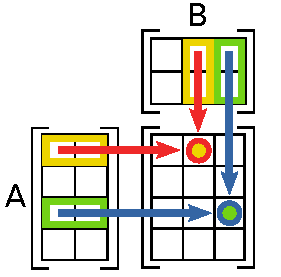
\includegraphics[width=0.3\textwidth]{matrix_multiplication.pdf}
    \caption{Mnożenie macierzy, źródło: Wikipedia.}
\end{figure}

\begin{remark}
    Mnożenie macierzy nie jest przemienne, jest za to łączne i obustronnie rozdzielne względem dodawania.
\end{remark}

\begin{fact}
    Zbiór $M_{m \times n}(\KK)$ macierzy o wymiarach $m \times n$ i elementach z ciała przemiennego $\KK$, $|\KK| \geq 2$ tworzy przestrzeń wektorową nad ciałem $\KK$.
\end{fact}

\begin{fact}
    Elementem neutralnym mnożenia macierzy kwadratowych jest macierz jednostkowa\footnote{jeśli macierz $A_{m\times n}$ nie jest kwadratowa, to również zachodzi $I'M = M$ oraz $M = I''M$ dla pewnych macierzy jednostkowych $I', I''$, lecz $I' \neq I''$ (są różnych wymiarów).}.
\end{fact}

\begin{fact}
    Zachodzi równość
    \[ (AB)^T = B^T A^T. \]
\end{fact}

        \subsection{Wyznacznik macierzy}
        \begin{definition}
    Inwersja w permutacji $\sigma \in S_n$ to taka para $\sigma(i), \sigma(j)$, że
    \[ i < j, \qquad \sigma(i) > \sigma(j). \]
\end{definition}

\begin{definition}
    Znak permutacji $\sigma$ to
    \[ \eps(\sigma) = (-1)^{(\text{liczba inwersji w } \sigma)}. \]
    Funkcję $\eps$ nazywamy symbolem Leviego-Civity.
\end{definition}

Jeśli $\eps(\sigma) = 1$, to permutacja $\sigma$ jest \vocab{parzysta}, a jeśli  $\eps(\sigma) = -1$, to jest \vocab{nieparzysta}.

\begin{fact}
    \label{f:sign of transposition}
    Każda transpozycja (zamiana miejscami) dwóch różnych elementów permutacji zmienia jej znak.
\end{fact}
\begin{proof}
    Weźmy permutację wraz z poniższymi oznaczeniami:
    \[ \sigma = (\underbrace{\sigma_1, \sigma_2, \ldots, \sigma_{i-1}}_A, \sigma_i, \underbrace{\sigma_{i+1}, \ldots, \sigma_{j-1}}_B, \sigma_j, \underbrace{\sigma_{j+1}, \ldots, \sigma_{n-1}, \sigma_n}_A). \]
    Zamieniając $\sigma_i$ oraz $\sigma_j$, nie zmienia się liczba inwersji zawierających dowolny element $\sigma_k \in A$. Nie zmieni się również liczba inwersji zawierających dowolny element $\sigma_k \in B$, który jest większy lub mniejszy jednocześnie od $\sigma_i$ i $\sigma_j$.

    Dla pozostałych elementów $\sigma_k \in B$, jeśli istnieje inwersja $(\sigma_i, \sigma_k)$, to istnieje również $(\sigma_k, \sigma_j)$, a jeśli istnieje inwersja $(\sigma_j, \sigma_k)$, to istnieje również $(\sigma_k, \sigma_i)$. Tak więc jedyną inwersją, która zmienia parzystość ogólnej liczby inwersji --- i tym samym $\eps(\sigma)$ --- jest inwersja $(\sigma_i, \sigma_j)$, która istnieje przed transpozycją, albo po niej.
\end{proof}

\begin{definition}
    \label{d:determinant}
    Wyznacznik macierzy kwadratowej $A$ to taki element ciała, że
    \[ \det A = \sum_{\sigma\in S_n} \eps(\sigma)a_{1\sigma(1)}a_{2\sigma(2)}\cdots a_{n\sigma(n)}. \]
    Oznaczamy $\det
    \left[\begin{smallmatrix}
        \cdots \\ \cdots \\ \cdots
    \end{smallmatrix}\right] =
    \left|\begin{smallmatrix}
        \cdots \\ \cdots \\ \cdots
    \end{smallmatrix}\right|$.
\end{definition}

\begin{theorem}[własności wyznaczników]
    \label{t:determinant properties}
    Dla macierzy kwadratowej $A = [a_{ij}] \in \sM_{n\times n}(\KK)$ zachodzi:
    \begin{enumerate}
        \item $\det A = \det A^T$,
        \item $\det I_n = 1$,
        \item jeśli istnieje zerowy wiersz (lub kolumna) to $\det A = 0$,
        \item jeśli pomnożymy jeden wiersz (lub kolumnę) przez skalar $\alpha$, to wyznacznik również będzie $\alpha$ razy większy,
        \item $\det \alpha A = (\det A) ^ \alpha$,
        \item \label{t:p:determinant of a matrix with sum} jeśli $A = [k_1, \ldots, k_j' + k_j'', \ldots, k_n]$, gdzie $k_i$ są wierszami (lub kolumnami), to
              \[ \det A = \det [k_1, \ldots, k_j', \ldots, k_n] + \det [k_1, \ldots, k_j'', \ldots, k_n], \]
        \item przestawienie dwóch wierszy macierzy zmienia znak wyznacznika na przeciwny,
        \item \label{t:p:determinant of a matrix with same rows} jeśli macierz ma dwa jednakowe wiersze (lub kolumny) to $\det A = 0$,
        \item wyznacznik nie zmieni się, jeśli do wiersza (albo kolumny) dodamy kombinację liniową pozostałych wierszy (kolumn).
    \end{enumerate}
\end{theorem}
\begin{proof} ~
    \begin{enumerate}
        \item Wszystkich par elementów w permutacji $\sigma \in S_n$ jest $n(n-1)$. Jeśli $(\sigma_i, \sigma_j)$ jest inwersją w $\sigma$, to w $\sigma^{-1}$ nią nie jest, a skoro $2\mid n(n-1)$, to $\eps(\sigma) = \eps(\sigma^{-1})$. Pozostałe czynniki sumowanych iloczynów zostaną takie same (jedynie w innej kolejności).
        \item Dla permutacji identycznościowej dany w definicji iloczyn jest równy $1$, dla każdej innej permutacji jest równy $0$.
        \item W każdym z sumowanych iloczynów występuje $0$ jako czynnik.
        \item W każdym z sumowanych iloczynów występuje jeden dodatkowy skalar $\alpha$.
        \item Wniosek z poprzedniego.
        \item Dowód podobny do poprzednich dwóch.
        \item Wynika z faktu \ref{f:sign of transposition}.
        \item Wniosek z poprzedniego, ponieważ $d = -d \implies d = 0$.
        \item Stwierdzenie jest prawdziwe, jeśli wyznacznik nie zmieni się, gdy do jednego wiersza (lub kolumny) dodamy inny (uzasadnienie przez indukcję). Ten fakt można udowodnić, łącząc punkty \ref{t:p:determinant of a matrix with sum} i \ref{t:p:determinant of a matrix with same rows} (jeden z wyznaczników będzie zerowy).
    \end{enumerate}
\end{proof}

\begin{theorem}
    Wyznacznik macierzy $2 \times 2$ jest równy
    \[ \det\begin{bmatrix}
        a_{11} & a_{12} \\
        a_{21} & a_{22}
    \end{bmatrix} = a_{11}a_{22} - a_{12}a_{21}. \]
\end{theorem}
\begin{proof}
    Prosty, z definicji.
\end{proof}

\begin{theorem}[reguła Sarrusa]
    Wyznacznik macierzy $3 \times 3$ jest równy
    \[ \det\begin{bmatrix}
        a_{11} & a_{12} & a_{13} \\
        a_{21} & a_{22} & a_{23} \\
        a_{31} & a_{32} & a_{33}
    \end{bmatrix} = \begin{aligned}[t] &a_{11}a_{22}a_{33} + a_{12}a_{23}a_{31} + a_{13}a_{21}a_{32} \\
                                       &- a_{13}a_{22}a_{31} - a_{11}a_{23}a_{32} - a_{12}a_{21}a_{33}.\end{aligned} \]
\end{theorem}
\begin{proof}
    Prosty, z definicji.
\end{proof}

Regułę Sarrusa bardzo łatwo zapamiętać: wystarczy przepisać na koniec macierzy dwie pierwsze kolumny i liczyć podobnie jak macierz $2 \times 2$.
\[ \begin{bNiceArray}{cc}
    a_{11} & a_{12} \\
    a_{21} & a_{22}
    \CodeAfter
        \tikz \draw [very thick, ForestGreen, opacity=0.4]
        (1-1.north west) -- (2-2.south east);
        \tikz \draw [very thick, Red, opacity=0.3]
        (1-2.north east) -- (2-1.south west);
\end{bNiceArray}
\qquad
\begin{bNiceArray}{ccc|cc}
    a_{11} & a_{12} & a_{13} & a_{11} & a_{12} \\
    a_{21} & a_{22} & a_{23} & a_{21} & a_{22} \\
    a_{31} & a_{32} & a_{33} & a_{31} & a_{32}
    \CodeAfter
        \tikz \draw [very thick, ForestGreen, opacity=0.4]
        (1-1.north west) -- (3-3.south east)
        (1-2.north west) -- (3-4.south east)
        (1-3.north west) -- (3-5.south east);
        \tikz \draw [very thick, Red, opacity=0.3]
        (1-3.north east) -- (3-1.south west)
        (1-4.north east) -- (3-2.south west)
        (1-5.north east) -- (3-3.south west);
\end{bNiceArray} \]

\begin{theorem}[Cauchy'ego]
    \label{t:det is multiplicative}
    Dla dowolnych macierzy $A, B \in \sM_{n\times n}(\KK)$ zachodzi
    \[ \det(A\cdot B) = \det A \cdot \det B. \]
\end{theorem}

\begin{definition}
    Minor stopnia $k$ macierzy $A_{m\times n}$ to wyznacznik podmacierzy kwadratowej $k\times k$ powstałej przez wykreślenie $n-k$ kolumn oraz $m-k$ wierszy.
\end{definition}

Jeśli $A_{n\times n}$ jest macierzą kwadratową, to wyznacznik macierzy powstałej przez wykreślenie $i$-tego wiersza i $j$-tej kolumny nazywamy \vocab{minorem odpowiadającym} elementowi $a_{ij}$ macierzy $A$ i oznaczamy $M_{ij}$.

\begin{definition}
    Dopełnienie algebraiczne elementu $a_{ij}$ macierzy kwadratowej $A = [a_{ij}]_{m\times n}$ to skalar
    \[ A_{ij} = (-1)^{i+j}M_{ij}. \]
\end{definition}

\begin{theorem}[rozwinięcie Laplace'a]
    \label{t:Laplace}
    Niech $A = [a_{ij}]_{n\times n}$ będzie macierzą kwadratową. Wtedy dla każdego ustalonego $i \in \{1,2\ldots,n\}$
    \[ \det A = \sum_{j=1}^n a_{ij}A_{ij} \]
    i dla każdego ustalonego $j \in \{1,2\ldots,n\}$
    \[ \det A = \sum_{i=1}^n a_{ij}A_{ij}. \]
\end{theorem}
\begin{proof}
    Dla wygody w oznaczeniach udowodnimy rozwinięcie wzdłuż pierwszego wiersza, $i = 1$. Weźmy taką permutację $\tau^j$, że permutuje ona zbiór $\{1, \ldots, n\} \setminus \{j\}$. Oznaczmy
    \[ \sigma^* = (j, \tau^j_1, \tau^j_2, \ldots, \tau^j_{j-1}, \tau^j_{j+1}, \ldots, \tau^j_{n}). \]
    Zauważmy, że $\eps(\sigma^*) = (-1)^{j-1} \eps(\tau^j)$. Teraz wystarczy ustalić $j$; z definicji wyznacznika (\ref{d:determinant}) mamy
    \begin{align*}
        \det A &= \sum_{\sigma\in S_n} \left(\eps(\sigma) \prod_{i=1}^n a_{i\sigma(i)}\right) = \sum_{\sigma\in S_n} \left(a_{1\sigma(1)} \cdot \eps(\sigma) \prod_{i=2}^n a_{i\sigma(i)}\right) = \\
        &= \sum_{j=1}^n \left(a_{1j} \sum_{\sigma^*} \left(\eps(\sigma^*) \prod_{i=2}^n a_{i\sigma^*(i)}\right)\right) = \\
        &= \sum_{j=1}^n \left(a_{1j} \sum_{\tau^j} \left((-1)^{j-1}\eps(\tau^j) \prod_{\substack{i=1\\i\neq j}}^n a_{i\tau^j(i)}\right)\right) = \\
        &= \sum_{j=1}^n \left(a_{1j} \left((-1)^{j-1} M_{1j}\right)\right) = \\
        &= \sum_{j=1}^n a_{1j} A_{1j}.
    \end{align*}

    Wiemy, że $\det A = \det A^T$ (z \ref{t:determinant properties}), więc możemy rozwijać również wzdłuż kolumn.
\end{proof}

\begin{corollary}
    \label{c:determinant in triangular matrix}
    Wyznacznik macierzy trójkątnej jest równy iloczynowi elementów na jej przekątnej.
\end{corollary}
\begin{proof}
    Wystarczy rozwijać wyznacznik wzdłuż pierwszej kolumny.
\end{proof}

        \subsection{Rząd macierzy}
        \begin{theorem}
    \label{t:rank}
    Maksymalna liczba liniowo niezależnych kolumn (wektorów z $\KK^m$) dowolnej macierzy $A \in M_{m\times n}(\KK)$ jest równa maksymalnej liczbie liniowo niezależnych wierszy (wektorów z $\KK^n$).
\end{theorem}
\begin{proof}
    TODO
\end{proof}

\begin{definition}
    \label{d:rank}
    Rząd macierzy to maksymalna liczba liniowo niezależnych kolumn (lub wierszy). Rząd macierzy $A$ oznaczamy przez $\rank (A)$.
\end{definition}

Z twierdzenia \ref{t:rank} i definicji \ref{d:rank} wynika, że
\[ \rank(A) = \rank(A^T). \]

\begin{definition}
    Macierz schodkowa to macierz, której pierwsze niezerowe elementy (schodki) kolejnych niezerowych wierszy znajdują się w coraz dalszych kolumnach, a wiersze zerowe umieszczone są najniżej.
\end{definition}

\begin{fact}
    Rząd macierzy schodkowej jest równy liczbie jej schodków.
\end{fact}

\begin{definition}
    Operacje elementarne na macierzach to:
    \begin{itemize}
        \item zamiana miejscami wierszy (kolumn) macierzy,
        \item dodanie do wiersza (kolumny) kombinacji liniowej pozostałych wierszy (kolumn),
        \item pomnożenie wiersza przez niezerowy skalar.
    \end{itemize}
    Jeśli macierz $B$ można otrzymać z macierzy $A$ za pomocą operacji elementarnych, to mówimy, że te macierze są \vocab{równoważne} i oznaczamy $A \sim B$.
\end{definition}

\begin{fact}
    Rząd macierzy nie zmienia się pod wpływem operacji elementarnych.
\end{fact}
\begin{proof}
    Wynika z twierdzenia \ref{t:linear independence}.
\end{proof}

Każdą macierz można łatwo doprowadzić do postaci schodkowej, za pomocą metody \vocab{eliminacji Gaussa}, która polega na stosowaniu operacji elementarnych na wierszach, ,,pozbywając się'' niezerowych elementów z dolnego trójkąta. W ten sposób można odczytać jej rząd oraz, za pomocą wniosku \ref{c:determinant in triangular matrix}, obliczyć jej wyznacznik (jeśli jest kwadratowa)\footnote{warto jednak zwrócić uwagę, że przy obliczaniu wyznacznika lepiej nie mnożyć wierszy i nie zamieniać ich miejscami, bo te operacje wpływają na wyznacznik}. 

\begin{example}
    Obliczyć wyznacznik macierzy
    \[ \begin{bmatrix}
        1 & 3 & 1 \\
        1 & 1 & -1 \\
        3 & 11 & 6
    \end{bmatrix}. \]
\end{example}
\begin{solution}
    \[ \begin{vmatrix}
        1 & 3 & 1 \\
        1 & 1 & -1 \\
        3 & 11 & 6
    \end{vmatrix} = \begin{vNiceMatrix}[create-medium-nodes]
        \CodeBefore[create-cell-nodes]
            \begin{tikzpicture}[name suffix = -medium]
                \node [highlight = (2-1) (2-3)] {} ;
                \node [highlight = (3-1) (3-3)] {} ;
            \end{tikzpicture}
        \Body
        1 & 3 & 1 \\
        0 & -2 & -2 \\
        0 & 2 & 3
    \end{vNiceMatrix} = \begin{vNiceMatrix}[create-medium-nodes]
        \CodeBefore[create-cell-nodes]
            \tikz[name suffix = -medium] \node [highlight = (3-1) (3-3)] {} ;
        \Body
        1 & 3 & 1 \\
        0 & -2 & -2 \\
        0 & 0 & 1
    \end{vNiceMatrix} = -2 \]
\end{solution}

\begin{theorem}
    \label{t:rank = max order of nonzero minor}
    Rząd macierzy $A$ jest równy największemu ze stopni niezerowych minorów tej macierzy.
\end{theorem}
\begin{proof}
    TODO
\end{proof}

\begin{example}
    Obliczyć rząd macierzy
    \[ A = \begin{bmatrix}
        1 & 3 & 4 \\
        3 & 4 & 1 \\
        1 & 2 & 7 \\
        3 & 5 & -1
    \end{bmatrix}. \]
\end{example}
\begin{solution}
    Obliczmy minor
    \[ \begin{vmatrix}
        1 & 3 & 4 \\
        3 & 4 & 1 \\
        3 & 5 & -1
    \end{vmatrix} = \begin{vmatrix}
        1 & 3 & 4 \\
        3 & 4 & 1 \\
        0 & 1 & -2
    \end{vmatrix} = (-8) + 0 + 12 - 0 - 1 - (-18) = 21 \neq 0. \]
    Ten minor jest niezerowy i jednocześnie ma największy stopień (bo wykreśliliśmy tylko jeden wiersz), więc na mocy twierdzenia \ref{t:rank = max order of nonzero minor} $\rank A = 3$.

    Dla pewności można pokazać również inną metodę --- eliminację Gaussa:
    \[ \begin{bmatrix}
        1 & 3 & 4 \\
        3 & 4 & 1 \\
        1 & 2 & 7 \\
        3 & 5 & -1
    \end{bmatrix} \sim \begin{bmatrix}
        1 & 3 & 4 \\
        0 & -5 & -11 \\
        0 & -1 & 3 \\
        0 & -4 & -13
    \end{bmatrix} \sim \begin{bmatrix}
        1 & 3 & 4 \\
        0 & 0 & -26 \\
        0 & -1 & 3 \\
        0 & 0 & -25
    \end{bmatrix} \sim \begin{bmatrix}
        1 & 3 & 4 \\
        0 & -1 & 3 \\
        0 & 0 & 1 \\
        0 & 0 & 0 \\
    \end{bmatrix} \]
    \[ \therefore \rank A = \rank \left[\begin{smallmatrix}
        1 & 3 & 4 \\
        0 & -1 & 3 \\
        0 & 0 & 1 \\
        0 & 0 & 0 \\
    \end{smallmatrix}\right] = 3. \]
\end{solution}

        \subsection{Macierz odwrotna}
        \begin{definition}
    \label{d:inverse matrix}
    Macierz odwrotna $A^{-1}$ do macierzy kwadratowej $A_{n\times n}$ to taka macierz, że
    \[ A\cdot A^{-1} = A^{-1}\cdot A = I_n. \]
    Jeśli taka macierz istnieje, to mówimy, że $A$ jest macierzą \vocab{odwracalną}.
\end{definition}

\begin{theorem}
    \label{t:invertible matrix}
    Jeśli macierz $A_{n\times n}$ jest odwracalna, to
    \begin{enumerate}
        \item $\det A \neq 0$ oraz $\det (A^{-1}) = (\det A)^{-1}$,
        \item $A^{-1} = \frac{1}{\det A} (A^D)^T$, gdzie $A^D$ jest macierzą dopełnień algebraicznych macierzy~$A$.
    \end{enumerate}
\end{theorem}
\begin{proof}
    \begin{enumerate}
        \item Z definicji macierzy odwrotnej (\ref{d:inverse matrix})
            \[ \begin{aligned} A\cdot A^{-1} =& I \\
                         \det(A\cdot A^{-1}) =& \det I = 1.
            \end{aligned} \]
            Na mocy twierdzenia Cauchy'ego (\ref{t:det is multiplicative}) otrzymujemy
            \[ \det A \cdot \det (A^{-1}) = 1, \]
            z czego wynika teza.
        \item Weźmy macierz $B$ taką, że
            \[ B = \det A^{-1} \cdot (A^D)^T, \]
            to znaczy, że dla każdego $i,j$ zachodzi
            \[ b_{ij} = \det A^{-1} \cdot A_{ji}, \]
            Obliczmy teraz macierz $C = AB$:
            \[ \begin{aligned}
                c_{ij} &= \sum_{k=1}^n a_{ik} b_{kj} \\
                       &= \sum_{k=1}^n a_{ik}\cdot\det A^{-1}\cdot A_{jk} \\
                       &= \det A^{-1}\sum_{k=1}^n a_{ik}\cdot A_{jk}.
            \end{aligned} \]
            Z rozwinięcia Laplace'a (\ref{t:Laplace}) otrzymujemy, że $c_{ij} = 1$ jeśli $i = j$ oraz $c_{ij} = 0$ w przeciwnym wypadku (TODO). W takim razie $C = I$, więc $B = A^{i-1}$.
    \end{enumerate}
\end{proof}

\begin{definition}
    Macierz osobliwa to macierz $A$, której wyznacznik jest zerowy. W innym wypadku $A$ jest macierzą nieosobliwą.
\end{definition}

Na podstawie twierdzenia \ref{t:invertible matrix} łatwo zauważyć, że pojęcie macierzy nieosobliwej jest równoznaczne macierzy odwracalnej, a macierzy osobliwej --- nieodwracalnej. Ponadto, jeśli macierz $A_{n\times n}$ jest nieosobliwa, to $\rank A = n$, a $A^{-1}, A^T, \alpha A, A^n$ również są macierzami nieosobliwymi.

Aby znaleźć macierz odwrotną, można oczywiście wykorzystać wzór
\[ A^{-1} = \frac{1}{\det A}(A^D)^T \]
z twierdzenia \ref{t:invertible matrix}, ale zwykle szybszą\footnote{na pewno w sensie złożoności obliczeniowej, w zadaniach to kwestia preferencji} metodą będzie eliminacja Gaussa, którą możemy wykorzystać wraz z poniższym faktem.

\begin{fact}
    Jeśli macierz kwadratowa $A$ jest odwracalna, to
    \[ \begin{bNiceArray}{cSc}A & I\end{bNiceArray} \sim \begin{bNiceArray}{cSc}I & B\end{bNiceArray} \quad\implies\quad B = A^{-1}. \]
\end{fact}
\begin{proof}
    Aby zrozumieć poniższy dowód trzeba się zapoznać z treścią sekcji \nameref{s:linear map}.

    Łatwo udowodnić, że każda operacja elementarna może być rozumiana jako pewne odwzorowanie liniowe, a tym samym --- jako operacja pomnożenia przez pewną macierz (odwzorowania liniowego). Drugi fakt, z którego należy sobie zdać sprawę, to równość
    \[ X\begin{bNiceArray}{cSc}A & I\end{bNiceArray} = \begin{bNiceArray}{cSc}XA & XI\end{bNiceArray}, \]
    która wynika bezpośrednio z definicji mnożenia macierzy. Z tych dwóch stwierdzeń wynika
    \[ \begin{bNiceArray}{cSc}A & I\end{bNiceArray} \sim \begin{bNiceArray}{cSc}X_1A & X_1I\end{bNiceArray} \sim \begin{bNiceArray}{cSc}X_2X_1A & X_2X_1I\end{bNiceArray} \sim \ldots \sim \begin{bNiceArray}{cSc}A^{-1}A & A^{-1}I\end{bNiceArray} = \begin{bNiceArray}{cSc}I & A^{-1}\end{bNiceArray}, \]
    gdzie $A^{-1}$ jest niejako ciągiem odwzorowań liniowych $X_i$, które wykonujemy podczas eliminacji Gaussa.
\end{proof}

\begin{example}
    \label{ex:inverse matrix}
    Znaleźć macierz odwrotną do macierzy
    \[ A = \begin{bmatrix}
        1 & 4 & 6 \\
        2 & 5 & 3 \\
        0 & 1 & 4
    \end{bmatrix}. \]
\end{example}
\begin{solution}
    \begin{align*}
        &\begin{bNiceArray}{cccIccc}
            1 & 4 & 6 & 1 & 0 & 0 \\
            2 & 5 & 3 & 0 & 1 & 0 \\
            0 & 1 & 4 & 0 & 0 & 1
        \end{bNiceArray} \sim \begin{bNiceArray}{cccIccc}
            1 & 4 & 6 & 1 & 0 & 0 \\
            0 & -3 & -9 & -2 & 1 & 0 \\
            0 & 1 & 4 & 0 & 0 & 1
        \end{bNiceArray} \sim \begin{bNiceArray}{cccIccc}
            1 & 4 & 6 & 1 & 0 & 0 \\
            0 & 1 & 3 & \frac{2}{3} & \frac{-1}{3} & 0 \\
            0 & 1 & 4 & 0 & 0 & 1
        \end{bNiceArray} \\ \sim &\begin{bNiceArray}{cccIccc}
            1 & 4 & 6 & 1 & 0 & 0 \\
            0 & 1 & 3 & \frac{2}{3} & \frac{-1}{3} & 0 \\
            0 & 0 & 1 & \frac{-2}{3} & \frac{1}{3} & 1
        \end{bNiceArray} \sim \begin{bNiceArray}{cccIccc}
            1 & 0 & -6 & \frac{-5}{3} & \frac{4}{3} & 0 \\
            0 & 1 & 3 & \frac{2}{3} & \frac{-1}{3} & 0 \\
            0 & 0 & 1 & \frac{-2}{3} & \frac{1}{3} & 1
        \end{bNiceArray} \sim \begin{bNiceArray}{cccIccc}
            1 & 0 & -6 & \frac{-5}{3} & \frac{4}{3} & 0 \\
            0 & 1 & 0 & \frac{8}{3} & \frac{-4}{3} & -3 \\
            0 & 0 & 1 & \frac{-2}{3} & \frac{1}{3} & 1
        \end{bNiceArray} \\ \sim &\begin{bNiceArray}{cccIccc}
            1 & 0 & 0 & \frac{-17}{3} & \frac{10}{3} & 6 \\
            0 & 1 & 0 & \frac{8}{3} & \frac{-4}{3} & -3 \\
            0 & 0 & 1 & \frac{-2}{3} & \frac{1}{3} & 1
        \end{bNiceArray},
    \end{align*}
    a więc
    \[ A^{-1} = \frac{1}{3}\begin{bmatrix}
                            -17 & 10 & 18 \\
                            8 & -4 & -9 \\
                            -2 & 1 & 3
    \end{bmatrix}. \]

    Możemy zweryfikować swoje obliczenia, znajdując macierz odwrotną metodą macierzy dopełnień algebraicznych.
    \begin{align*} A^{-1} &= \frac{1}{5 \cdot 4 + 6 \cdot 2 - 4 \cdot 2 \cdot 4 - 3}\begin{bmatrix}
            5 \cdot 4 - 3 & -(2 \cdot 4) & 2 \\
            -(4 \cdot 4 - 6) & 4 & -(1) \\
            4 \cdot 3 - 6 \cdot 5 & -(3 - 6 \cdot 2) & 5 - 4 \cdot 2
        \end{bmatrix}^T \\ &= \frac{1}{-3}\begin{bmatrix}
            17 & -8 & 2 \\
            -10 & 4 & -1 \\
            -18 & 9 & -3
        \end{bmatrix}^T = \frac{1}{3}\begin{bmatrix}
            -17 & 10 & 18 \\
            8 & 4 & 9 \\
            -2 & 1 & 3
        \end{bmatrix}.
    \end{align*}
\end{solution}

Macierz odwrotną można znaleźć również rozwiązując układ równań liniowych
\[ A \cdot X = B, \]
wtedy $A^{-1} \cdot B = X$ --- o czym więcej w następnej sekcji.

    \section{Układy równań liniowych}
    Układ $m$ równań liniowych z $n$ niewiadomymi $x_1, \ldots, x_n$ w postaci
\begin{equation}
    \label{eq:linear system}\begin{cases}
    a_{11}x_1 + a_{12}x_2 + \ldots + a_{1n}x_n &= b_1 \\
    a_{21}x_1 + a_{22}x_2 + \ldots + a_{2n}x_n &= b_2 \\
    \cdots \\
    a_{m1}x_1 + a_{m2}x_2 + \ldots + a_{mn}x_n &= b_m \\
\end{cases}\end{equation}
możemy reprezentować jako równanie macierzy. Macierz
\[ A = \begin{bNiceMatrix}
    a_{11} & a_{12} & \Cdots & a_{1n} \\
    a_{21} & a_{22} & \Cdots & a_{2n} \\
    \Vdots & \Vdots & \Ddots & \Vdots \\
    a_{m1} & a_{m2} & \Cdots & a_{mn}
\end{bNiceMatrix} \]
nazywamy \vocab{macierzą główną} (macierzą współczynników) układu \ref{eq:linear system}, a macierze
\[ B = \begin{bNiceMatrix}
    b_1 \\ b_2 \\ \Vdots \\ b_m
\end{bNiceMatrix}, \qquad X = \begin{bNiceMatrix}
    x_1 \\ x_2 \\ \Vdots \\ x_n
\end{bNiceMatrix} \]
nazywamy odpowiednio \vocab{kolumną wyrazów wolnych} oraz \vocab{kolumną niewiadomych}. Połączenie macierzy $A$ i $B$
\[ \begin{bNiceArray}{cSc}A & B\end{bNiceArray}  = \begin{bNiceArray}{cccIc}
    a_{11} & \Cdots & a_{1n} & b_1 \\
    \Vdots & \Ddots & \Vdots & \Vdots \\
    a_{m1} & \Cdots & a_{mn} & b_m
\end{bNiceArray} \]
jest \vocab{macierzą uzupełnioną} tego układu. Wtedy układ \ref{eq:linear system} zapisujemy macierzowo jako
\[ A \cdot X = B. \]

\begin{definition}
    Układ jednorodny to taki układ równań liniowych, że kolumna wyrazów wolnych jest zerowa.
\end{definition}

\begin{definition}
    Układ jest:
    \begin{itemize}
        \item \vocab{oznaczony}, jeśli ma jedno rozwiązanie,
        \item \vocab{nieoznaczony}, jeśli ma więcej niż jedno rozwiązanie,
        \item \vocab{sprzeczny}, jeśli nie ma rozwiązań.
    \end{itemize}
\end{definition}

\begin{definition}
    Układ kwadratowy to układ równań liniowych, w którym liczba niewiadomych jest równa liczbie równań (czyli macierz główna jest kwadratowa).
\end{definition}

\begin{definition}
    Układ Cramera to układ kwadratowy, w którym wyznacznik macierzy głównej jest niezerowy, $\det A \neq 0$.
\end{definition}

\begin{theorem}[Cramera]
    \label{t:Cramer}
    Jeśli dany układ jest układem Cramera, to jest oznaczony oraz
    \[ x_j = \frac{D_{x_j}}{\det A}, \]
    gdzie $D_{x_j}$ jest wyznacznikiem macierzy powstałej przez zastąpienie $j$-tej kolumny macierzy głównej $A$ kolumną wyrazów wolnych $B$.
\end{theorem}
\begin{proof}
    Pierwsze stwierdzenie jest prawdziwe, ponieważ jeśli $\det A \neq 0$, to kolumny tworzą bazę pewnej przestrzeni liniowej, do której należy kolumna $B$, więc na mocy twierdzenia \ref{t:explicit coefficients} jest ona jednoznacznie wyznaczona przez kombinację liniową kolumn z~$A$~(a współczynniki tej kombinacji liniowej są właśnie kolumną niewiadomych $X$).

    Oznaczając $j$-tą kolumną $A$ jako $\mathbf{a_j}$ oraz $B = \mathbf{b}$, na mocy poprzedniego akapitu równanie
    \[ x_1\mathbf{a_1} + x_2\mathbf{a_2} + \ldots + x_n\mathbf{a_n} = \mathbf{b} \]
    spełnia dokładnie jeden wektor $\mathbf{x}$. Zatem
    \[ D_{x_j} = \det(\mathbf{a_1}, \ldots, \mathbf{b}, \ldots, \mathbf{a_n}) = \det(\mathbf{a_1}, \ldots, \sum_{i=1}^n x_i\mathbf{a_i}, \ldots, \mathbf{a_n}). \]
    Z własności wyznaczników (\ref{t:determinant properties}) wynika, że wyznacznika nie zmieni odjęcie od pewnej kolumny innej kolumny przemnożonej przez skalar (nawet zerowy), więc
    \[ D_{x_j} = \det(\mathbf{a_1}, \ldots, x_j\mathbf{a_j}, \ldots, \mathbf{a_n}) = x_j\det(\mathbf{a_1}, \ldots, \mathbf{a_j}, \ldots, \mathbf{a_n}) = x_j \det A, \]
    \[ \therefore x_j = \frac{D_{x_j}}{\det A}. \]
\end{proof}

\begin{theorem}[Kroneckera-Capellego]
    \label{t:Kronecker-Cappelli}
    Układ $AX = B$ ma co najmniej jedno rozwiązanie wtedy i tylko wtedy, gdy
    \[ \rank(A) = \rank(\begin{bNiceArray}{cSc}A & B\end{bNiceArray}). \]
\end{theorem}
\begin{proof}
    Oznaczając $j$-tą kolumną $A$ jako $\mathbf{a_j}$ oraz $B = \mathbf{b}$, mamy
    \[ x_1\mathbf{a_1} + x_2\mathbf{a_2} + \ldots + x_n\mathbf{a_n} = \mathbf{b}, \]
    a więc $X$ istnieje wtedy i tylko wtedy, gdy kolumna $B$ jest kombinacją liniową kolumn z~$A$~(a więc nie jest liniowo niezależna, ergo $\rank(A) = \rank(\begin{bNiceArray}{cSc}A & B\end{bNiceArray})$).
\end{proof}

\begin{theorem}
    \label{t:rankA = rankA|B = n}
    Układ $AX = B$ ma dokładnie jedno rozwiązanie wtedy i tylko wtedy, gdy
    \[ \rank(A) = \rank(\begin{bNiceArray}{cSc}A & B\end{bNiceArray}) = n, \]
    gdzie $n$ jest liczbą niewiadomych.
\end{theorem}
\begin{proof}
    Jak poprzednio, lecz z wykorzystaniem twierdzenia \ref{t:explicit coefficients}.
\end{proof}

Prosty wniosek z tego twierdzenia jest taki, że jeśli $\rank(A) = \rank(\begin{bNiceArray}{cSc}A & B\end{bNiceArray})$, ale $\rank(A) \neq n$, to układ jest nieoznaczony, a jego rozwiązania zależą od $n - \rank(A)$ parametrów\footnote{Jeśli układ jest określony nad ciałem $\RR$ lub $\CC$, to układ nieoznaczony ma nieskończenie wiele rozwiązań.}.

Układy równań liniowych można łatwo rozwiązać eliminacją Gaussa w podobny sposób, jak robiliśmy to, szukając macierzy odwrotnej w przykładzie \ref{ex:inverse matrix}.

\begin{example}
    Rozwiązać układ równań
    \[ \begin{cases}
        x + 3y - z &= 2 \\
        2x - 3z &= -5 \\
        3x + 2y - 3z &= -1
    \end{cases}. \]
\end{example}
\begin{solution}
    \[ \begin{bNiceArray}{cccIc}
        1 & 3 & -1 & 2 \\
        2 & 0 & -3 & -5 \\
        3 & 2 & -3 & -1
    \end{bNiceArray} \sim \begin{bNiceArray}{cccIc}
        1 & 3 & -1 & 2 \\
        0 & -6 & -1 & -9 \\
        0 & -7 & 0 & -7
    \end{bNiceArray} \sim \begin{bNiceArray}{cccIc}
        1 & 3 & -1 & 2 \\
        0 & 1 & -1 & -2 \\
        0 & 1 & 0 & 1
    \end{bNiceArray} \sim \begin{bNiceArray}{cccIc}
        1 & 3 & -1 & 2 \\
        0 & 1 & -1 & -2 \\
        0 & 0 & 1 & 3
    \end{bNiceArray} \]
    Rząd macierzy jest równy liczbie zmiennych, więc (na mocy twierdzenia \ref{t:rankA = rankA|B = n}) układ jest oznaczony. Teraz możemy kontynuować przekształcenia, aby otrzymać macierz $\begin{bNiceArray}{cSc}I & X\end{bNiceArray}$, ale w praktyce łatwiej będzie teraz wrócić do układu równań. Mamy więc
    \[ z = 3, \]
    \[ y - z = -2 \implies y = -2 + 3 = 1, \]
    \[ x + 3x - z = 2 \implies x = 2 - 3 + 3 = 2. \]
\end{solution}

    \section{Geometria analityczna}
    W tej sekcji skupimy się na przestrzeni $\RR^3(\RR)$, w której wektory będziemy interpretować często jako punkty lub wektory zaczepione w środku układu współrzędnych. Przez $\RR^n$ oznaczymy zbiór punktów, a przez $\overrightarrow{\RR^n}$ zbiór wektorów. W przestrzeni $\RR^3$ osie \vocab{prawoskrętnego}\footnote{to znaczy zgodnego z regułą prawej ręki --- wnętrze obracającej się dłoni zakreśla łuk od osi $OX$ do $OY$, przy czym kciuk ma zwrot zgodny z osią $OZ$} układu współrzędnych $(x, y, z)$ będą rozpięte przez \vocab{wersory} (wektory o jednostkowej długości):
\[ \mathbf{\hat{i}} = (1, 0, 0), \quad \mathbf{\hat{j}} = (0, 1, 0), \quad \mathbf{\hat{k}} = (0, 0, 1). \]

\begin{definition}
    \label{d:Euclidean metric}
    Metryka euklidesowa w $\RR^n$ to funkcja $d : \RR^n \times \RR^n \to \RR$, która dla punktów $P = (x_1, x_2, \ldots, x_n), Q = (y_1, y_2, \ldots, y_n)$ jest zdefiniowana jako
    \[ d(P, Q) = \sqrt{\sum_{i = 1}^n (y_i - x_i)^2}. \]
    Wartość tej funkcji dla punktów $X, Y$ to \vocab{odległość euklidesowa} tych punktów.
\end{definition}

\begin{definition}
    Norma euklidesowa w $\RR^n$ to funkcja $\Vert\cdot\Vert : \overrightarrow{\RR^n} \to \RR_{\geq 0}$, która dla wektora $v = [v_1, v_2, \ldots, v_n]$ jest zdefiniowana jako
    \[ \Vert v\Vert = \sqrt{\sum_{i=1}^n v_i^2}. \]
    Wartość normy wektora $v$ to \vocab{długość} tego wektora.
\end{definition}

Łatwo zauważyć korelację między tymi dwoma wzorami: dla dwóch punktów $P, Q$, wektor $\overrightarrow{PQ}$ jest równy
\[ \ol{PQ} = [y_1 - x_1, \ldots, y_n - x_n], \]
więc
\[ d(P, Q) = \Vert\overrightarrow{PQ}\Vert. \]

\begin{definition}
    Iloczyn skalarny wektorów $u = [u_1, \ldots, u_n]$ i $v = [v_1, \ldots, v_n]$ w przestrzeni $\RR^n$ to liczba
    \[ u \circ v = \sum_{i=1}^n u_iv_i. \]
\end{definition}

\begin{fact}
    Jeśli $U^T$ jest jednokolumnową macierzą powstałą z wektora $u$, a $V$ to jednowierszową macierz powstała z wektora $v$, to
    \[ u \circ v = U^T \cdot V. \]
\end{fact}

\begin{fact}
    Dla każdego wektora $v \in \RR^n$ zachodzi
    \[ \sqrt{v \circ v} = \Vert v \Vert. \]
\end{fact}

Jeśli dla przestrzeni wektorowej $\RR^n$ określimy iloczyn skalarny wektorów, to taka przestrzeń jest \vocab{przestrzenią euklidesową}, którą oznaczamy przez $E_n$. Warto zauważyć, że taki iloczyn skalarny jest łączny, przemienny, zgodny z mnożeniem przez skalar oraz rozdzielny względem dodawania.

\begin{theorem}[Cauchy'ego-Schwarza]
    Dla dowolnych wektorów $\mathbf{u}, \mathbf{v} \in E_n$ zachodzi nierówność
    \[ |\mathbf{u} \circ \mathbf{v}| \leq \Vert \mathbf{u} \Vert \cdot \Vert \mathbf{v} \Vert, \]
    przy czym równość zachodzi wtedy i tylko wtedy, gdy wektory są liniowo zależne.
\end{theorem}
\begin{proof}
    Twierdzenie jest trywialne, jeśli któryś z wektorów jest zerowy, dlatego przyjmijmy $\mathbf{u}, \mathbf{v} \neq \ol{0}$. Dla dowolnego $\alpha \in \RR$ mamy
    \[ 0 \leq \Vert\mathbf{u} - \alpha\mathbf{v}\Vert^2 = (\mathbf{u} - \alpha\mathbf{v}) \circ (\mathbf{u} - \alpha\mathbf{v}) = \mathbf{u} \circ \mathbf{u} - 2\alpha(\mathbf{u} \circ \mathbf{v}) + \alpha^2(\mathbf{v} \circ \mathbf{v}). \]
    Podstawiając $\alpha = (\mathbf{u} \circ \mathbf{v})(\mathbf{v} \circ \mathbf{v})^{-1}$ otrzymamy
    \[ 0 \leq (\mathbf{u} \circ \mathbf{u}) - (\mathbf{v} \circ \mathbf{v})^{-1}(\mathbf{u} \circ \mathbf{v})^2 \]
    \[ (\mathbf{v} \circ \mathbf{v})^{-1}(\mathbf{u} \circ \mathbf{v})^2 \leq (\mathbf{u} \circ \mathbf{u}) \]
    \[ (\mathbf{u} \circ \mathbf{v})^2 \leq (\mathbf{u} \circ \mathbf{u})(\mathbf{v} \circ \mathbf{v}) \]
    \[ (\mathbf{u} \circ \mathbf{v})^2 \leq \Vert \mathbf{u} \Vert^2 \cdot \Vert \mathbf{v} \Vert^2 \]
    \[ |\mathbf{u} \circ \mathbf{v}| \leq \Vert \mathbf{u} \Vert \cdot \Vert \mathbf{v} \Vert. \]
    Równość zachodzi tylko w przypadku, gdy $\alpha = 0$, czyli gdy $\mathbf{u}, \mathbf{v}$ są liniowo zależne.
\end{proof}

\begin{corollary}[Nierówność trójkąta]
    \label{c:triangle inequality}
    Dla dowolnych wektorów $\mathbf{u}, \mathbf{v} \in E_n$ zachodzi nierówność
    \[ \Vert \mathbf{u} + \mathbf{v} \Vert  \leq \Vert \mathbf{u} \Vert + \Vert \mathbf{v} \Vert, \]
\end{corollary}
\begin{proof}
    Z nierówności Cauchy'ego-Schwarza wynika, że
    \begin{align*}
        \mathbf{u} \circ \mathbf{v} &\leq \sqrt{\mathbf{u} \circ \mathbf{u}} \cdot \sqrt{\mathbf{v} \circ \mathbf{v}} \\
        \mathbf{u} \circ \mathbf{u} + 2 \cdot \mathbf{u} \circ \mathbf{v} + \mathbf{v} \circ \mathbf{v} &\leq \mathbf{u} \circ \mathbf{u} + 2 \cdot \sqrt{\mathbf{u} \circ \mathbf{u}} \cdot \sqrt{\mathbf{v} \circ \mathbf{v}} + \mathbf{v} \circ \mathbf{v} \\
        (\mathbf{u} + \mathbf{v}) \circ (\mathbf{u} + \mathbf{v}) &\leq (\sqrt{\mathbf{u} \circ \mathbf{u}} + \sqrt{\mathbf{v} \circ \mathbf{v}})^2 \\
        \Vert \mathbf{u} + \mathbf{v} \Vert^2  &\leq (\Vert \mathbf{u} \Vert + \Vert \mathbf{v} \Vert)^2 \\
        \Vert \mathbf{u} + \mathbf{v} \Vert  &\leq \Vert \mathbf{u} \Vert + \Vert \mathbf{v} \Vert.
    \end{align*}
\end{proof}

\begin{definition}
    \label{d:angle between vectors}
    Kąt między niezerowymi wektorami $\mathbf{u}, \mathbf{v} \in E_n$ to taka liczba $\sphericalangle(\mathbf{u}, \mathbf{v}) = \varphi \in [0, \pi]$, że
    \[ \cos\varphi = \frac{\mathbf{u} \circ \mathbf{v}}{\Vert \mathbf{u} \Vert \cdot \Vert \mathbf{v} \Vert}. \]
\end{definition}

Jeśli $\sphericalangle(\mathbf{u}, \mathbf{v}) = \frac{\pi}{2}$, to wektory są \vocab{prostopadłe} $\mathbf{u} \perp \mathbf{v}$, a jeśli $\sphericalangle(\mathbf{u}, \mathbf{v}) = 0$ lub $\pi$, to są \vocab{równoległe} $\mathbf{u} \parallel \mathbf{v}$. Przyjmujemy, że wektor zerowy jest prostopadły i równoległy do wszystkich innych wektorów.

\begin{fact}
    Dla dowolnych wektorów $\mathbf{u}, \mathbf{v} \in E_n$
    \[ \mathbf{u} \perp \mathbf{v} \quad \iff \quad \mathbf{u} \circ \mathbf{v} = 0 \]
\end{fact}
\begin{proof}
    Wynika z definicji.
\end{proof}

Oczywiście $\mathbf{u} \parallel \mathbf{v}$ wtedy i tylko wtedy, gdy wektory $\mathbf{u}, \mathbf{v}$ są liniowo zależne.

\subsection{Przestrzeń trójwymiarowa}
\begin{fact}
    Trójka liniowo niezależnych wektorów $\mathbf{u}, \mathbf{v}, \mathbf{w} \in E_3$ tworzy układ prawoskrętny, jeśli
    \[ \begin{vmatrix}
        \mathbf{u}_1 & \mathbf{u}_2 & \mathbf{u}_3 \\
        \mathbf{v}_1 & \mathbf{v}_2 & \mathbf{v}_3 \\
        \mathbf{w}_1 & \mathbf{w}_2 & \mathbf{w}_3
    \end{vmatrix} > 0. \]
\end{fact}
\begin{proof}[Uzasadnienie]
    Jest to intuicyjnie prawdziwe --- jeśli zamienimy wiersze ze sobą, to układ wektorów stanie się lewoskrętny i jednocześnie (z własności wyznaczników \ref{t:determinant properties}) wyznacznik macierzy będzie przeciwny. Podobnie, jeśli zmienimy zwrot danego wektora, to układ stanie się lewoskrętny, a wyznacznik macierzy będzie przeciwny.

    Dociekliwy Czytelnik może zaznajomić się z dowodem zawartym w artykule ,,\textit{\href{https://sites.math.washington.edu/~marshall/math_136/right-hand-rule.pdf}{A Simple Proof of the Right-Hand Rule}}'' autorstwa Fuchang Gao.
\end{proof}

\begin{definition}
    \label{d:cross product}
    Iloczyn wektorowy to takie działanie $\times : (\overrightarrow{E_3})^2 \to \overrightarrow{E_3}$, że:
    \begin{enumerate}
        \item jeśli $\mathbf{u} \parallel \mathbf{v}$, to $\mathbf{u} \times \mathbf{v} = \ol{0}$,
        \item w przeciwnym wypadku $\mathbf{u} \times \mathbf{v} = \mathbf{w}$, gdzie
            \begin{itemize}
                \item $\Vert\mathbf{w}\Vert = \Vert\mathbf{u}\Vert \cdot \Vert\mathbf{v}\Vert\cdot\sin\sphericalangle(\mathbf{u}, \mathbf{v})$,
                \item $\mathbf{w} \perp \mathbf{u}$ oraz $\mathbf{w} \perp \mathbf{v}$,
                \item wektory $\mathbf{u}, \mathbf{v}, \mathbf{w}$ tworzą układ prawoskrętny.
            \end{itemize}
    \end{enumerate}
\end{definition}

\begin{theorem}
    Dla dowolnych wektorów $\mathbf{u}, \mathbf{v} \in E_3$
    \[ \mathbf{u} \times \mathbf{v} = \left[\begin{vmatrix}
        \mathbf{u}_2 & \mathbf{u}_3 \\
        \mathbf{v}_2 & \mathbf{v}_3
    \end{vmatrix}, \begin{vmatrix}
        \mathbf{u}_3 & \mathbf{u}_1 \\
        \mathbf{v}_3 & \mathbf{v}_1
    \end{vmatrix}, \begin{vmatrix}
        \mathbf{u}_1 & \mathbf{u}_2 \\
        \mathbf{v}_1 & \mathbf{v}_2
    \end{vmatrix}\right]\]
\end{theorem}
\begin{proof}
    Żmudny, ale prosty; z definicji.
\end{proof}

W praktyce łatwiej stosować (zapamiętać) ,,wzór''
\begin{equation} \label{eq:easy cross product}
    \mathbf{u} \times \mathbf{v} = \begin{vmatrix}
        \mathbf{\hat{i}} & \mathbf{\hat{j}} & \mathbf{\hat{k}} \\
        \mathbf{u}_1 & \mathbf{u}_2 & \mathbf{u}_3 \\
        \mathbf{v}_1 & \mathbf{v}_2 & \mathbf{v}_3
    \end{vmatrix} = \mathbf{\hat{i}}\begin{vmatrix}
        \mathbf{u}_2 & \mathbf{u}_3 \\
        \mathbf{v}_2 & \mathbf{v}_3
    \end{vmatrix} + \mathbf{\hat{j}}\begin{vmatrix}
        \mathbf{u}_3 & \mathbf{u}_1 \\
        \mathbf{v}_3 & \mathbf{v}_1
    \end{vmatrix} + \mathbf{\hat{k}}\begin{vmatrix}
        \mathbf{u}_1 & \mathbf{u}_2 \\
        \mathbf{v}_1 & \mathbf{v}_2
    \end{vmatrix}
\end{equation}

Warto zauważyć, że iloczyn wektorowy jest antyprzemienny ($\mathbf{u} \times \mathbf{v} = -\mathbf{v} \times \mathbf{u})$, zgodny z mnożeniem przez skalar oraz rozdzielny względem dodawania.

\begin{fact}
    Dla dowolnych wektorów $\mathbf{u}, \mathbf{v} \in E_3$
    \[ \mathbf{u} \parallel \mathbf{v} \quad \iff \quad \mathbf{u} \times \mathbf{v} = \ol{0} \]
\end{fact}
\begin{proof}
    Wynika z definicji.
\end{proof}

\begin{theorem}
    \label{t:area of parallelogram}
    Dla dowolnych wektorów $\mathbf{u}, \mathbf{v} \in E_3$ liczba $\Vert\mathbf{u}\times\mathbf{v}\Vert$ jest (skierowanym) polem równoległoboku rozpiętego przez wektory $\mathbf{u}, \mathbf{v}$.
\end{theorem}
\begin{proof}
    Z definicji iloczynu wektorowego (\ref{d:cross product}) mamy
    \[ \Vert\mathbf{u}\times\mathbf{v}\Vert = \Vert\mathbf{u}\Vert\cdot\Vert\mathbf{v}\Vert\cdot\sin\sphericalangle(\mathbf{u}, \mathbf{v}), \]
    czyli iloczyn długości obu boków oraz sinusa kąta między nimi, który istotnie jest równy polu równoległoboku.
\end{proof}

Prosty wniosek z tego twierdzenia jest taki, że pole trójkąta rozpiętego przez wektory $\mathbf{u}, \mathbf{v}$ jest równe $\frac{1}{2}\Vert\mathbf{u}\times\mathbf{v}\Vert$.

Działanie $(\mathbf{u}\times\mathbf{v}) \circ \mathbf{w}$ nazywamy \vocab{iloczynem mieszanym}.

\begin{theorem}
    \label{t:volume of parallelepiped}
    Dla dowolnych wektorów $\mathbf{u}, \mathbf{v}, \mathbf{w} \in E_3$ liczba $\left((\mathbf{u}\times\mathbf{v}) \circ \mathbf{w}\right)$ jest (skierowaną) objętością równoległościanu rozpiętego przez wektory $\mathbf{u}, \mathbf{v}, \mathbf{w}$.
\end{theorem}
\begin{proof}
    Z definicji kąta między wektorami (\ref{d:angle between vectors}) mamy
    \[ (\mathbf{u}\times\mathbf{v}) \circ \mathbf{w} = \Vert\mathbf{u}\times\mathbf{v}\Vert \cdot \Vert\mathbf{w}\Vert \cdot \cos\phi, \]
    gdzie $\Vert\mathbf{u}\times\mathbf{v}\Vert$ to pole równoległoboku rozpiętego przez wektory $\mathbf{u}, \mathbf{v}$, jak na rysunku poniżej.

    \begin{center}
        \begin{tikzpicture}[vect/.style={->,>=latex',thick,MainColor1}]
            \def\a{3}
            \def\bx{1.7} \def\by{.8}
            \def\cx{.9} \def\cy{2.5}
            \tkzDefPoints{0/0/O, \a/0/A, \bx/\by/B, \cx/\cy/C, \cx+\a/\cy/D,
                          \bx/\by/B, \a+\bx/\by/A', \cx+\bx/\cy+\by/C', \cx+\a+\bx/\cy+\by/D',
                          0/\cy/V}
            \tkzDrawPolygon(D,A,A',D',C',C)
            \tkzDrawSegments(D,D')
            \tkzDrawSegments[thin](O,V)
            \tkzDrawSegments[dashed](B,C' B,A')
            \tkzDrawSegments[vect](O,A O,C)
            \tkzDrawSegments[dashed,vect](O,B)
            \tkzMarkAngle[size=1.4](C,O,V)
            \tkzLabelAngle[font=\scriptsize](C,O,V){$\phi$}
            \tkzLabelSegment[font=\scriptsize, below](O,A){$\mathbf{u}$}
            \tkzLabelSegment[font=\scriptsize, below, pos=.7](O,B){$\mathbf{v}$}
            \tkzLabelSegment[font=\scriptsize, right](O,C){$\mathbf{w}$}
        \end{tikzpicture}
    \end{center}
\end{proof}

Prosty wniosek z tego twierdzenia jest taki, że objętość czworościanu rozpiętego przez wektory $\mathbf{u}, \mathbf{v}, \mathbf{w}$ jest równa $\frac{1}{6}|(\mathbf{u}\times\mathbf{v}) \circ \mathbf{w}|$.

\begin{fact}
    \label{f:triple product}
    Dla dowolnych wektorów $\mathbf{u}, \mathbf{v}, \mathbf{w} \in E_3$
    \[ (\mathbf{u}\times\mathbf{v}) \circ \mathbf{w} = \begin{vmatrix}
        \mathbf{u}_1 & \mathbf{u}_2 & \mathbf{u}_3 \\
        \mathbf{v}_1 & \mathbf{v}_2 & \mathbf{v}_3 \\
        \mathbf{w}_1 & \mathbf{w}_2 & \mathbf{w}_3
    \end{vmatrix}. \]
    Jest to prostszy sposób na liczenie objętości równoległościanu.
\end{fact}
\begin{proof}
    Łatwo zauważyć zależność między rozwinięciem Laplace'a (\ref{t:Laplace}) oraz wzorem~\ref{eq:easy cross product}.
\end{proof}

\subsubsection{Równanie płaszczyzny w przestrzeni}
Płaszczyznę jednoznacznie wyznaczają trzy niewspółliniowe punkty (lub wyznaczone przez nie dwa wektory). Płaszczyznę jednoznacznie wyznaczyć może również jeden niezerowy wektor, zwany \vocab{wektorem normalnym}; jest on prostopadły do wyznaczanej płaszczyzny.

\paragraph{Równanie parametryczne płaszczyzny} Jeśli $P_0 = (x_0, y_0, z_0) \in \pi$ oraz $\mathbf{u} = [\mathbf{u}_1, \mathbf{u}_2, \mathbf{u}_3]$, $\mathbf{v} = [\mathbf{v}_1, \mathbf{v}_2, \mathbf{v}_3] \in E_3$ są liniowo niezależne i równoległe do płaszczyzny $\pi$, to
\begin{equation} \pi : \begin{cases}
    x = x_0 + s\mathbf{u}_1 + t\mathbf{v}_1 \\
    y = y_0 + s\mathbf{u}_2 + t\mathbf{v}_2 \\
    z = z_0 + s\mathbf{u}_3 + t\mathbf{v}_3
\end{cases} \qquad s, t \in \RR \end{equation}
jest równaniem parametrycznym płaszczyzny. Wtedy każdy punkt płaszczyzny jest po prostu punktem $P_0$, który został przesunięty o pewien wektor równoległy do płaszczyzny.

\paragraph{Równanie normalne płaszczyzny} Jeśli $n = [A, B, C]$ jest wektorem normalnym płaszczyzny $\pi$ oraz $P_0 = (x_0, y_0, z_0) \in \pi$, to
\[ \pi : [x - x_0, y - y_0, z - z_0] \circ [A, B, C] = 0 \]
czyli
\begin{equation}
    \pi : A(x - x_0) + B(y - y_0) + C(z - z_0) = 0
\end{equation}
nazywamy równaniem normalnym płaszczyzny $\pi$. Wtedy każdy punkt $P_1 \in \pi$ jest taki, że wektor $\overrightarrow{P_0P_1}$ jest prostopadły do wektora normalnego, czyli równoległy do płaszczyzny.

\paragraph{Równanie ogólne płaszczyzny} Równanie normalne można wymnożyć do równania ogólnego
\begin{equation}
    \pi : Ax + By + Cz + D = 0.
\end{equation}

\paragraph{Równanie odcinkowe płaszczyzny} Jeśli $a, b, c \in \RR$ są niezerowe, to
\begin{equation}
    \pi : \frac{x}{a} + \frac{y}{b} + \frac{z}{c} = 1
\end{equation}
jest równaniem odcinkowym płaszczyzny. Taka płaszczyzna przecina się z osiami układu współrzędnych w punktach $(a, 0, 0), (0, b, 0), (0, 0, c)$; tak więc nie każda płaszczyzna ma równianie odcinkowe.

\subsubsection{Równanie prostej w przestrzeni}
Prostą jednoznacznie wyznaczają dwa punkty (lub jeden wyznaczony przez nie wektor). Prosta jest również jednoznacznie wyznaczona przez przecięcie dwóch nierównoległych płaszczyzn.

\paragraph{Równanie parametryczne prostej} Jeśli $P_0 = (x_0, y_0, z_0) \in l$ oraz $\mathbf{v} = [\mathbf{v}_1, \mathbf{v}_2, \mathbf{v}_3] \in E_3$ jest niezerowym wektorem równoległym do prostej $l$, to
\begin{equation} l : \begin{cases}
    x = x_0 + t\mathbf{v}_1 \\
    y = y_0 + t\mathbf{v}_2 \\
    z = z_0 + t\mathbf{v}_3
\end{cases} \qquad t \in \RR \end{equation}
jest równaniem parametrycznym prostej. Wektor $\mathbf{v}$ nazywamy wektorem \vocab{kierunkowym} (lub tworzącym, rozpinającym) prostej $l$.

\paragraph{Równanie kierunkowe prostej} Jeśli $P_0 = (x_0, y_0, z_0) \in l$ oraz $\mathbf{v} = [a, b, c] \in E_3$ jest równoległy do prostej $l$ i $a, b, c \in \RR$ są niezerowe, to
\begin{equation}
    l : \frac{x - x_0}{a} = \frac{y - y_0}{b} = \frac{z - z_0}{c}
\end{equation}
jest równaniem kierunkowym prostej.

\paragraph{Równanie krawędziowe prostej} Niech
\[ \pi_1 : A_1x + B_1y + C_1z + D_1 = 0, \pi_2 : A_2x + B_2y + C_2z + D_2 = 0. \]
Jeśli $\pi_1$ nie jest równoległa z $\pi_2$, to równanie krawędziowe prostej ma postać
\begin{equation}
    l : \begin{cases}
        A_1x + B_1y + C_1z + D_1 = 0 \\
        A_2x + B_2y + C_2z + D_2 = 0
    \end{cases}.
\end{equation}

\begin{remark*}
    Jeśli chcemy łatwo przejść z równania krawędziowego do parametrycznego, to wystarczy zauważyć, że $n_1 = [A_1, B_1, C_1], n_2 = [A_2, B_2, C_2]$ są wektorami normalnymi płaszczyzn. Chcemy znaleźć więc wektor (kierunkowy), który leży na obu tych płaszczyznach, a więc jest prostopadły do obu wektorów normalnych. Tę własność ma wektor $\mathbf{v} = n_1 \times n_2$.
\end{remark*}

\subsection{Odległości}
Zdefiniowaliśmy już odległość między dwoma punktami w definicji \ref{d:Euclidean metric}. Bez formalnego wyprowadzenia będziemy używać pojęcia odległości również w kontekście odległości między punktem a płaszczyzną, punktem a prostą, prostą a płaszczyzną czy między płaszczyznami lub prostymi. Taka odległość będzie najmniejszą odległością między pewnym punktem jednej figury oraz pewnym punktem drugiej figury.
\[ d(\Phi, \Psi) = \min_{A \in \Phi, B \in \Psi} d(A, B) \]
Z twierdzenia Pitagorasa wynika, że wektor między tymi dwoma punktami będzie prostopadły do powierzchni obu danych figur.

\begin{theorem}[Odległość punktu od płaszczyzny]
    \label{t:distance between point and plane}
    Odległość punktu $Q = (x_1, y_1, z_1)$ od płaszczyzny $\pi : Ax + Bx + Cx + D = 0$ jest równa
    \[ d(Q, \pi) = \frac{|Ax_1 + By_1 + Cz_1 + D|}{\sqrt{A^2 + B^2 + C^2}}. \]
\end{theorem}
\begin{proof}
    Niech prosta $l$ będzie prostopadła do płaszczyzny $\pi$ oraz niech $Q \in l$. Taka prosta jest równoległa do wektora normalnego $n = [A, B, C]$, więc
    \[ l : \begin{cases}
        x = x_1 + At \\
        y = y_1 + Bt \\
        z = z_1 + Ct
    \end{cases} \qquad t \in \RR. \]
    Niech $Q' = \pi \cap l$ będzie punktem przecięcia prostej $l$ i płaszczyzny $\pi$. Podstawiamy równanie prostej do równania płaszczyzny:
    \begin{align*}
        Q' \in l &: A(x_1 + tA) + B(y_1 + tB) + C(z_1 + tC) + D = 0 \\
        Q' \in l &: t = \frac{Ax_1 + By_1 + Cz_1 + D}{-(A^2 + B^2 + C^2)}
    \end{align*}
    Mamy więc
    \[ d(Q, Q') = \sqrt{(tA)^2 + (tB)^2 + (tC)^2} = |t| \cdot \sqrt{A^2 + B^2 + C^2} = \frac{|Ax_1 + By_1 + Cz_1 + D|}{\sqrt{A^2 + B^2 + C^2}}. \]
\end{proof}

Jeśli szukamy odległości między dwoma płaszczyznami, to wystarczy sprawdzić, czy są one równoległe (to znaczy, czy ich wektory normalne są równoległe). Jeśli nie, to odległość jest oczywiście zerowa; w przeciwnym wypadku wystarczy wziąć dowolny punkt z jednej płaszczyzny i znaleźć odległość między tym punktem a drugą płaszczyzną.

\begin{theorem}[Odległość punktu od prostej]
    Odległość punktu $Q$ od prostej $l$ jest równa
    \[ d(Q, l) = \frac{\Vert \mathbf{v} \times \overrightarrow{LQ}\Vert}{\Vert\mathbf{v}\Vert}, \]
    gdzie $\mathbf{v}$ jest wektorem kierunkowym prostej $l$, a $L \in l$.
\end{theorem}
\begin{proof}
    Mamy $l : (x, y, z) = L + t\mathbf{v}$. Na podstawie twierdzenia \ref{t:area of parallelogram}, pole równoległoboku rozpiętego przez wektory $\mathbf{v}, \overrightarrow{LQ}$ jest równe
    \[ \Vert \mathbf{v} \times \overrightarrow{LQ} \Vert. \]
    \begin{center}
        \begin{tikzpicture}[scale=.8]
            \tkzDefPoints{2/5/Q,-1/3/L,1/2/L'}
            \tkzDefPointBy[projection = onto L--L'](Q) \tkzGetPoint{H}
            \tkzDefPointBy[translation = from L to L'](Q) \tkzGetPoint{Q'}
            \tkzFillPolygon[color=MainColor1!10](L,L',Q',Q)
            \tkzDrawLine[add= .5 and .5](L,L')
            \tkzDrawSegment[dashed](Q,H)
            \tkzDrawSegments[MainColor1, vector style](L,Q L,L')
            \tkzDrawSegments[dotted, MainColor1](L',Q' Q,Q')
            \tkzDrawPoints(Q, L)
            \tkzLabelSegment[swap](L,L'){$\mathbf{v}$}
            \tkzLabelPoints[above right](Q)
            \tkzLabelPoints[below left](L)
        \end{tikzpicture}
    \end{center}
    Ze standardowego wzoru na pole równoległoboku jest ono również równe
    \[ \Vert \mathbf{v} \Vert \cdot d(Q, l), \]
    z czego wynika teza.
\end{proof}

Jeśli dwie proste są równoległe, to odległość między nimi można obliczyć przez wzięcie dowolnego punktu z jednej prostej i obliczenie jego odległości od drugiej prostej. Jeśli proste się przecinają, to odległość między nimi jest zerowa. Sytuacja się komplikuje, jeśli dane dwie proste nie są równoległe lub przecinające się (to znaczy są \vocab{skośne}).

\begin{theorem}[Odległość prostych skośnych]
    \label{t:distance between lines}
    Niech $l_1, l_2$ są prostymi skośnymi. Odległość między nimi jest równa
    \[ d(l_1, l_2) = \frac{|(\mathbf{v} \times \mathbf{u}) \circ \overrightarrow{L_1L_2}|}{\Vert\mathbf{v}\times\mathbf{u}\Vert}, \]
    gdzie $\mathbf{v}, \mathbf{u}$ są odpowiednio wektorami kierunkowym prostych $l_1, l_2$, a $L_1 \in l_1$ i $L_2 \in l_2$.
\end{theorem}
\begin{proof}
    Mamy $l_1 : (x, y, z) = L_1 + t\mathbf{v}$ oraz $l_2 : (x, y, z) = L_2 + t\mathbf{u}$. Na podstawie twierdzenia \ref{t:volume of parallelepiped} objętość równoległościanu rozpiętego przez wektory $\mathbf{v}, \mathbf{u}, \overrightarrow{L_1L_2}$ jest równa
    \[ |(\mathbf{v} \times \mathbf{u}) \circ \overrightarrow{L_1L_2}|. \]
    Ze standardowego wzoru na objętość (tzn.\ pole podstawy $\cdot$ wysokość) jest ona również równa
    \[ \Vert\mathbf{v}\times\mathbf{u}\Vert \cdot d(l_1, l_2), \]
    z czego wynika teza.
\end{proof}

\subsection{Przykłady}
\begin{example}[Współliniowość punktów]
    Sprawdź, czy punkty $A = (1, 0, 2), B = (3, 1, -1), C = (-1, -1, 5)$ są współliniowe.
\end{example}
\begin{solution}
    Punkty $A, B, C$ są współliniowe wtedy i tylko wtedy, gdy wektory $\overrightarrow{AB}, \overrightarrow{AC}$ są współliniowe, czyli rozpinają równoległobok o zerowym polu. Na podstawie twierdzenia \ref{t:area of parallelogram} wystarczy obliczyć
    \[ \left\Vert\overrightarrow{AB}\times\overrightarrow{AC}\right\Vert = \Vert[2, 1, -3] \times [-2, -1, 3]\Vert = \Vert[3 - 3, 6 - 6, -2 + 2]\Vert = 0, \]
    z czego wynika, że punkty $A, B, C$ są współliniowe.
\end{solution}

\begin{example}[Współpłaszczyznowość punktów]
    Sprawdź, czy punkty $A = (0, 2, 2), B = (2, 1, 0), C = (3, -1, 2), D = (1, -2, 3)$ są współpłaszczyznowe.
\end{example}
\begin{solution}
    Punkty $A, B, C, D$ są współpłaszczyznowe wtedy i tylko wtedy, gdy wektory $\overrightarrow{AB}, \overrightarrow{AC}, \overrightarrow{AD}$ rozpinają równoległościan o zerowej objętości. Na podstawie twierdzenia \ref{t:volume of parallelepiped} i faktu \ref{f:triple product} wystarczy obliczyć
    \[ \begin{vmatrix}
        \overrightarrow{AB} \\
        \overrightarrow{AC} \\
        \overrightarrow{AD}
    \end{vmatrix} = \begin{vmatrix}
        2 & -1 & -2 \\
        3 & -3 & 0 \\
        1 & -4 & 1
    \end{vmatrix} = -6 + 24 - 6 + 3 = 15 \neq 0, \]
    z czego wynika, że punkty $A, B, C, D$ nie są współpłaszczyznowe.
\end{solution}

\begin{example}[Wzajemne położenie prostych, odległość]
    Zbadaj wzajemne położenie prostych
    \[ l_1 : \begin{cases}
        x = 1 - 3t \\
        y = 2 - 6t \\
        z = 3 - 5t
    \end{cases} \quad t \in \RR, \qquad
    l_2 : \begin{cases}
        x = 2 + t \\
        y = -1 + 2t \\
        z = 4 + 2t
    \end{cases} \quad t \in \RR \]
    oraz oblicz odległość między nimi.
\end{example}
\begin{solution}
    Zaczniemy od sprawdzenia, czy proste są równoległe. Weźmy wektory kierunkowe tych prostych i obliczmy ich iloczyn wektorowy. Mamy
    \[ [-3, -6, -5] \times [1, 2, 2] = \begin{vmatrix}
        \mathbf{\hat{i}} & \mathbf{\hat{j}} & \mathbf{\hat{k}} \\
        -3 & -6 & -5 \\
        1 & 2 & 2
    \end{vmatrix} = [-12 + 10, -5 + 6, -6 + 6] = [-2, 1, 0] \neq \ol{0}, \]
    więc proste nie są równoległe. Odległość między nimi, zgodnie z twierdzeniem \ref{t:distance between lines}, jest równa
    \[ d(l_1, l_2) = \frac{|[-2, 1, 0] \circ [2-1, -1-2, 4-3]|}{\Vert[-2, 1, 0]\Vert} = \frac{|-2 - 3|}{\sqrt{5}} = \sqrt{5}. \]
    Z tego wynika również, że proste są skośne; nie są przecinające się, bo $d(l_1, l_2) \neq 0$.
\end{solution}

\begin{example}[Wzajemne położenie prostych, wspólna płaszczyzna]
    Zbadaj wzajemne położenie prostych
    \[ l_1 : \begin{cases}
        x = t \\
        y = -2t \\
        z = 3t
    \end{cases} \quad t \in \RR, \qquad
    l_2 : \begin{cases}
        x = -1 + t \\
        y = 2 - t \\
        z = -3 + 4t
    \end{cases} \quad t \in \RR \]
    oraz wyznacz ich wspólną płaszczyznę (jeśli istnieje).
\end{example}
\begin{solution}
    Obliczmy najpierw iloczyn wektory wektorów kierunkowych danych prostych.
    \[ [1, -2, 3] \times [1, -1, 4] = \begin{vmatrix}
        \mathbf{\hat{i}} & \mathbf{\hat{j}} & \mathbf{\hat{k}} \\
        1 & -2 & 3 \\
        1 & -1 & 4
    \end{vmatrix} = [-8 + 3, 3 - 4, -1 + 2] = [-5, -1, 1] \]
    Widzimy więc, że proste nie są równoległe. Zamiast liczyć odległość między nimi (i tak stwierdzić, czy się przecinają), możemy spróbować znaleźć punkt przecięcia.
    \[ \begin{cases}
        t = -1 + s \\
        -2t = 2 - s \\
        3t = -3 + 4s
    \end{cases} \implies s = 0, t = -1. \]
    Z tego wynika, że punkt przecięcia istnieje, jest nim $P = (-1, 2, -3)$, więc proste nie są skośne, a więc tworzą płaszczyznę.

    Do tej płaszczyzny należą wektory kierunkowe prostych $l_1, l_2$, więc jej wektorem normalnym będzie ich iloczyn wektorowy. Podstawiając do równania normalnego płaszczyzny mamy
    \begin{align*}
        \pi :& -5(x - (-1)) -1(y - 2) + 1(z - (-3)) = 0 \\
             & -5x - 5 - y + 2 + z + 3 = 0 \\
             & -5x - y + z = 0
    \end{align*}
    co jest równaniem ogólnym płaszczyzny $\pi$.
\end{solution}

\begin{remark*}
    Jeśli chcemy znaleźć rzut prostokątny punktu $P$ na prostą $l$, to najłatwiej będzie znaleźć płaszczyznę $\pi$ zawierającą punkt $P$ i prostopadłą do prostej $l$ (wektor normalny szukanej płaszczyzny będzie wektorem kierunkowym prostej $l$). Następnie wystarczy znaleźć punkt przecięcia $\pi \cap l$.

    Podobnie, jeśli chcemy znaleźć rzut prostokątny punktu $P$ na płaszczyznę $\pi$, to należy znaleźć prostą $l$ taką, że $l \perp \pi$ oraz $P \in l$ (jak poprzednio, wektor kierunkowy szukanej prostej będzie wektorem normalnym płaszczyzny $\pi$).
\end{remark*}

Zastosowanie powyższej uwagi niech będzie ćwiczeniem dla Czytelnika\footnote{który z pewnością zauważył już, że wykorzystaliśmy ją w dowodzie twierdzenia \ref{t:distance between point and plane}}.

    \section{Odwzorowania liniowe} \label{s:linear map}
    \begin{definition}
    \label{d:linear map}
    Odwzorowanie
    \[ f : V \lthen W, \]
    gdzie $V, W$ są przestrzeniami liniowymi nad tym samym ciałem $\KK$ jest \vocab{liniowe}, jeśli
    \[ \dforall{u, v \in V} f(u + v) = f(u) + f(v) \]
    oraz
    \[ \dforall{v \in V, \alpha \in \KK} f(\alpha v) = \alpha f(v), \]
    to znaczy, kiedy jest \vocab{addytywne} oraz \vocab{jednorodne}.
\end{definition}

Podobnie jak w przypadku homomorfizmu grup (definicja \ref{d:homomorphism}), elementy przeciwne oraz neutralne są zachowywane. Analogicznie do równoważnej charakterystyki podprzestrzeni (fakt \ref{f:equivalent subspace characteristics}) warunki z powyższej definicji są równoważne warunkowi
\begin{equation}
    \label{eq:equivalent liner map condition}
    \dforall{\alpha, \beta \in \KK}\dforall{u, v \in V} f(\alpha u + \beta v) = \alpha f(u) + \beta f(v).
\end{equation}

\begin{corollary}[z równania \ref{eq:equivalent liner map condition}]
    \label{c:linear map is unique by the values f(B)}
    Odwzorowanie liniowe $f$ jest jednoznacznie określone przez wartości $f$ na wektorach bazowych dziedziny.
\end{corollary}
\begin{proof}
    Wzór \ref{eq:equivalent liner map condition} można rozszerzyć do większej liczby składników używając $(\alpha, \beta, \gamma, \ldots)$ oraz $(u, v, w, \ldots)$. Taka postać również będzie równoważna definicji \ref{d:linear map}. Możemy policzyć wartość $f$ dla każdego wektora, znając jego współrzędne w pewnej bazie $B$ oraz wartości $f$ dla wszystkich wektorów z tej bazy.
\end{proof}

\begin{definition}
    Jądro odwzorowania liniowego $f : V \lthen W$ to zbiór
    \[ \Ker f = f^{-1}(\{\ol{0}\}) = \{v \in V \mid f(v) = \ol{0}\}. \]
\end{definition}

\begin{definition}
    Obraz odwzorowania liniowego $f : V \lthen W$ to zbiór
    \[ \Im f = f(V) = \{w \in W \mid \exists v \in V : w = f(v)\}. \]
    Jeśli $B$ jest bazą przestrzeni $V$, to
    \[ \Im f = \Lin f(B). \]
\end{definition}

\begin{fact}
    Dla każdego odwzorowania liniowego $f : V \lthen W$, jądro $f$ jest podprzestrzenią $V$, a obraz $f$ jest podprzestrzenią $W$.
\end{fact}

Wymiar jądra pewnego odwzorowania $f$ nazywamy \vocab{zerowością} i oznaczamy $\nullity f$, a wymiar jego obrazu nazywamy \vocab{rzędem} i oznaczamy $\rank f$.

\begin{example}
    Weźmy odwzorowanie $f : \RR^3 \lthen \RR^2$ takie, że
    \[ f(x, y, z) = (x, y). \]
    Znajdźmy jądro i obraz tego odwzorowania.
    \[ \Ker f = \{(0, 0, z) : z \in \RR\}, \quad \dim = 1. \]
    \[ \Im f = \RR^2, \quad \dim = 2. \]
    Teraz weźmy $g : \RR^2 \lthen \RR^3$ takie, że
    \[ g(x, y) = (x, y, x + y). \]
    Znajdźmy jądro i obraz tego odwzorowania.
    \[ \Ker g = \{\ol{0}\}, \quad \dim = 0. \]
    \[ \Im g = \{(x, y, x+y) : x, y \in \RR\}, \quad \dim = 2. \]
\end{example}

\begin{theorem}[o rzędzie]
    \label{t:rank-nullity}
    Jeśli $V, W$ są skończenie wymiarowymi przestrzeniami wektorowymi nad ciałem $\KK$ oraz $f : V \lthen W$ jest odwzorowaniem liniowym, to
    \[ \nullity f + \rank f = \dim V, \]
    \[ \dim \Ker f + \dim \Im f = \dim V. \]
\end{theorem}
\begin{proof}
    Niech $n = \dim V$ oraz $k = \dim \Ker f$. Skoro $\Ker f$ jest podprzestrzenią przestrzeni $V$, to jeśli $n = k$, to dla każdego $\mathbf{v} \in V$ zachodzi $f(\mathbf{v}) = \ol{0}$, więc $\Im f = \{\ol{0}\}$, ergo teza jest spełniona. Dalej załóżmy więc, że $n > k$. Istnieje taka baza przestrzeni $V$, która ma postać
    \[ \{\mathbf{v}_1, \ldots, \mathbf{v}_k, \mathbf{u}_{k+1}, \ldots, \mathbf{u}_n\}, \]
    gdzie $\{\mathbf{v}_1, \ldots, \mathbf{v}_k\}$ jest bazą $\Ker f$. Weźmy dowolny wektor $\mathbf{v} \in V,$
    \[ \mathbf{v} = t_1\mathbf{v}_1 + \ldots + t_k\mathbf{v}_k + t_{k+1}\mathbf{u}_{k+1} + \ldots + t_n\mathbf{u}_n. \]
    Wtedy
    \begin{align*}
        \mathbf{w} = f(\mathbf{v}) &= f(t_1\mathbf{v}_1 + \ldots + t_k\mathbf{v}_k + t_{k+1}\mathbf{u}_{k+1} + \ldots + t_n\mathbf{u}_n) \\
            &= f(t_1\mathbf{v}_1) + \ldots + f(t_k\mathbf{v}_k) + f(t_{k+1}\mathbf{u}_{k+1}) + \ldots + f(t_n\mathbf{u}_n) \\
            &= t_1f(\mathbf{v}_1) + \ldots + t_kf(\mathbf{v}_k) + t_{k+1}f(\mathbf{u}_{k+1}) + \ldots + ft_n(\mathbf{u}_n) \\
            &= t_1(0) + \ldots + t_k(0) + t_{k+1}f(\mathbf{u}_{k+1}) + \ldots + ft_n(\mathbf{u}_n) \\
            &= t_{k+1}f(\mathbf{u}_{k+1}) + \ldots + ft_n(\mathbf{u}_n),
    \end{align*}
    więc
    \[ \Im f = \Lin\{f(\mathbf{u}_{k+1}), \ldots, f(\mathbf{u}_n)\}. \]
    Wystarczy już tylko udowodnić, że wektory $f(\mathbf{u}_{k+1}), \ldots, f(\mathbf{u}_n)$ są liniowo niezależne. Weźmy ciąg skalarów $(s_i)$ taki, że
    \begin{align*}
        s_{k+1}f(\mathbf{u}_{k+1}) + \ldots + s_nf(\mathbf{u}_n) &= \ol{0} \\
        f(s_{k+1}\mathbf{u}_{k+1}) + \ldots + f(s_n\mathbf{u}_n) &= \ol{0} \\
        f(s_{k+1}\mathbf{u}_{k+1} + \ldots + s_n\mathbf{u}_n) &= \ol{0}.
    \end{align*}
    Z tego wynika, że
    \[ (s_{k+1}\mathbf{u}_{k+1} + \ldots + s_n\mathbf{u}_n) \in \Ker f, \]
    więc $(s_{k+1}\mathbf{u}_{k+1} + \ldots + s_n\mathbf{u}_n) \in V$ możemy zapisać jako kombinację liniową wektorów $\mathbf{v}_1, \ldots, \mathbf{v}_k$. Zakładając, że ciąg $(s_i)$ jest niezerowy, mamy dwa sposoby zapisu jednego wektora z $V$, co stoi w sprzeczności z twierdzeniem \ref{t:explicit coefficients}. Z tego wynika, że $\forall i : s_i = 0$, więc wektory $f(\mathbf{u}_{k+1}), \ldots, f(\mathbf{u}_n)$ są liniowo niezależne, ergo
    \[ \dim \Im f = n - k \]
    \[ \rank f = \dim V - \nullity f. \]
\end{proof}

\begin{definition}
    Przy danych przestrzeniach wektorowych $V, W$ nad ciałem $\KK$, odwzorowanie liniowe $f : V \lthen W$ to:
    \begin{itemize}
        \item \vocab{monomorfizm}, jeśli jest injekcją,
        \item \vocab{epimorfizm}, jeśli jest surjekcją,
        \item \vocab{izomorfizm}, jeśli jest bijekcją,
        \item \vocab{endomorfizm}, jeśli $V = W$,
        \item \vocab{automorfizm}, jeśli jest endomorfizmem i izomorfizmem,
        \item \vocab{forma liniowa}, jeśli $W = \KK$.
    \end{itemize}
\end{definition}

\begin{theorem}
    Odwzorowanie liniowe $f : V \lthen W$ jest epimorfizmem wtedy i tylko wtedy, gdy $\dim\Im f = \dim W$.
\end{theorem}
\begin{proof}
    $\Im f$ jest podprzestrzenią $W$, więc wynika z twierdzenia \ref{t:dimU = dimV, U subspace V}.
\end{proof}

\begin{theorem}
    Odwzorowanie liniowe $f : V \lthen W$ jest monomorfizmem wtedy i tylko wtedy, gdy $\Ker f = \{\ol{0}\}$.
\end{theorem}
\begin{proof}
    Implikacja prawostronna jest trywialna, dlatego udowodnimy tylko lewostronną. Załóżmy przeciwnie, że istnieje takie $\mathbf{v}_1 \neq \mathbf{v}_2$, że
    \[ f(\mathbf{v}_1) = f(\mathbf{v}_2). \]
    Wtedy
    \[ f(\mathbf{v}_1) - f(\mathbf{v}_2) = f(\mathbf{v}_2) - f(\mathbf{v}_1) = \ol{0} \]
    \[ f(\mathbf{v}_1 - \mathbf{v}_2) = f(\mathbf{v}_2 - \mathbf{v}_1) = \ol{0}, \]
    co, skoro $\mathbf{v}_1 - \mathbf{v}_2 \neq \ol{0}$, przeczy założeniu $\Ker f = \{\ol{0}\}$.
\end{proof}

\begin{theorem}
    Jeśli $V, W$ są skończenie wymiarowymi przestrzeniami wektorowymi nad ciałem $\KK$, to ich izomorficzność jest równoważna równości ich wymiarów
    \[ V \sim W \quad \iff \quad \dim V = \dim W. \]
\end{theorem}
\begin{proof}
    Wynika z wniosku \ref{c:linear map is unique by the values f(B)}.
\end{proof}

\begin{theorem}
    Niech $V, W$ będą pewnymi przestrzeniami nad ciałem $\KK$, a $\sL(V, W)$ zbiorem wszystkich odwzorowań liniowych między nimi. Struktura $(\sL(V, W), \KK, +, \cdot)$ jest przestrzenią wektorową.
\end{theorem}
\begin{proof}
    Z definicji.
\end{proof}

\subsection{Macierze odwzorowań liniowych}
\begin{definition}
    \label{d:transformation matrix}
    Niech $B_V = (e_1, e_2, \ldots, e_n), B_W = (l_1, l_2, \ldots, l_m)$ będą pewnymi bazami odpowiednio przestrzeni $V, W$ nad ciałem $\KK$. Niech $f : V \lthen W$ będzie odwzorowaniem liniowym takim, że
    \begin{align*}
        f(e_1) &= a_{11}l_1 + a_{21}l_2 + \ldots + a_{m1}l_m, \\
        f(e_2) &= a_{12}l_1 + a_{22}l_2 + \ldots + a_{m2}l_m, \\
        \vdots \\
        f(e_n) &= a_{1n}l_1 + a_{2n}l_2 + \ldots + a_{mn}l_m.
    \end{align*}
    \vocab{Macierz odwzorowania liniowego} $f$ w bazach $B_V, B_W$ to macierz
    \[ M_f(B_V, B_W) = \begin{bNiceMatrix}
        a_{11} & a_{12} & \Cdots & a_{1n} \\
        a_{21} & a_{22} & \Cdots & a_{2n} \\
        \Vdots & \Vdots & \Ddots & \Vdots \\
        a_{m1} & a_{m2} & \Cdots & a_{mn}
    \end{bNiceMatrix}. \]
\end{definition}

\begin{fact}
    \label{f:matix form of linear map}
    Równanie $y = f(x)$ można zapisać w postaci macierzowej jako
    \[ \begin{bNiceMatrix}y_1 \\ y_2  \\ \Vdots \\ y_m\end{bNiceMatrix} = \begin{bNiceMatrix}
        a_{11} & a_{12} & \Cdots & a_{1n} \\
        a_{21} & a_{22} & \Cdots & a_{2n} \\
        \Vdots & \Vdots & \Ddots & \Vdots \\
        a_{m1} & a_{m2} & \Cdots & a_{mn}
    \end{bNiceMatrix}\begin{bNiceMatrix}x_1 \\ x_2  \\ \Vdots \\ x_n\end{bNiceMatrix}, \]
    gdzie $f : B_V \lthen B_W$ jest odwzorowaniem liniowym, $[a_{ij}]_{m\times n} = M_f(B_V, B_W)$ oraz
    \[ x = [x_1, x_2, \ldots, x_n]_{B_V}^T, \quad y = [y_1, y_2, \ldots, y_m]_{B_W}^T. \]
\end{fact}
\begin{proof}
    Skoro $x = [x_1, x_2, \ldots, x_n]_{B_V}^T$ oraz $y = [y_1, y_2, \ldots, y_m]_{B_W}^T$, to
    \[ x = x_1e_1 + x_2e_2 + \ldots + x_ne_n, \quad y = y_1l_1 + y_2l_2 + \ldots + y_ml_m, \]
    więc
    \begin{align}
        f(x) &= f(x_1e_1 + x_2e_2 + \ldots + x_ne_n) \nonumber \\
        f(x) &= x_1f(e_1) + x_2f(e_2) + \ldots + x_nf(e_n) \nonumber \\
        f(x) &= x_1\begin{bNiceMatrix}a_{11} \\ a_{21} \\ \Vdots \\ a_{m1}\end{bNiceMatrix}
            + x_2\begin{bNiceMatrix}a_{12} \\ a_{22} \\ \Vdots \\ a_{m2}\end{bNiceMatrix}
            + \ldots
            + x_n\begin{bNiceMatrix}a_{1n} \\ a_{2n} \\ \Vdots \\ a_{mn}\end{bNiceMatrix}
            \label{eq:matrix form of linear map - linear combination}
    \end{align}

    Mnożąc macierze jak w udowadnianej tezie otrzymalibyśmy
    \[ y = \begin{bNiceMatrix}
        a_{11}x_1 + a_{12}x_2 + \ldots + a_{1n}x_n \\
        a_{21}x_1 + a_{22}x_2 + \ldots + a_{2n}x_n \\
        \Vdots \\
        a_{m1}x_1 + a_{m2}x_2 + \ldots + a_{mn}x_n \\
    \end{bNiceMatrix}, \]
    czyli to samo co wyżej.
\end{proof}

Jeśli odwzorowanie $f$ jest endomorfizmem, to macierz tego odwzorowania w bazie $B$ oznaczamy jako $M_f(B)$.

\begin{theorem}
    Jeśli $f : V \lthen W$ będzie odwzorowaniem liniowym, a $B_V, B_W$ to bazy odpowiednio przestrzeni $V, W$, to
    \[ \rank f = \rank M_f(B_V, B_W). \]
\end{theorem}
\begin{proof}
    Przypomnijmy, że
    \[ \Im f = \{y \in W \mid \exists x \in V : y = f(x)\}. \]
    Korzystając z faktu \ref{f:matix form of linear map}, możemy przekształcić powyższe do
    \[ \Im f = \{M_f(B_V, B_W)\cdot x \mid x \in V\}, \]
    z czego wynika, że obraz przekształcenia $f$ jest tożsamy z przestrzenią rozpinaną przez kolumny macierzy $M_f(B_V, B_W)$ (zobacz równanie \ref{eq:matrix form of linear map - linear combination}). Z tego powodu również ich wymiary są równe.
\end{proof}

\begin{theorem}
    Niech $f, g : V \lthen W$ będą odwzorowaniami liniowymi, $B_V, B_W$ to bazy odpowiednio przestrzeni $V, W$ nad ciałem $\KK$, a $\alpha \in \KK$, to
    \begin{enumerate}
        \item $M_{f+g}(B_V, B_W) = M_f(B_V, B_W) + M_g(B_V, B_W)$,
        \item $M_{\alpha f}(B_V, B_W) = \alpha M_f(B_V, B_W)$,
    \end{enumerate}
\end{theorem}
\begin{proof}
    Z definicji.
\end{proof}

\begin{theorem}
    Niech $f : V \lthen W, g : W \lthen U$ będą odwzorowaniami liniowymi, a $B_V, B_W, B_U$ to bazy odpowiednio przestrzeni $V, W, U$, to
    \[ M_{g\circ f}(B_V, B_U) = M_g(B_W, B_U) + M_f(B_V, B_W). \]
\end{theorem}
\begin{proof}
    Z definicji oraz faktu \ref{f:matix form of linear map}.
\end{proof}

\begin{corollary}[z faktu \ref{f:matix form of linear map}]
    Endomorfizm $f : V \lthen V$ jest automorfizmem (bijekcją) wtedy i tylko wtedy, gdy macierz przekształcenia liniowego jest odwracalna (nieosobliwa). Łatwo również znaleźć przekształcenie odwrotne $f^{-1}$:
    \[ M_{f^{-1}}(B_2, B_1) = (M_f(B_1, B_2))^{-1}. \]
\end{corollary}

\begin{definition}
    Macierz przejścia $P_{B \lthen B'}$ od bazy $B = (e_1, e_2, \ldots, e_n)$ do bazy $B' = (e_1', e_2', \ldots, e_n')$ przestrzeni $V$ to macierz odwzorowania identycznościowego danej przestrzeni w bazach $B', B$,
    \[ P_{B\lthen B'} = M_{\opname{Id}_V}(B', B). \]
    Wtedy, jeśli $X, X'$ są wektorami kolumnowymi z $V$ względem baz $B, B'$, to
    \[ X = P_{B \lthen B'}X'. \]
\end{definition}

\begin{remark*}
    W powyżej opisanej macierzy $j$-tą kolumnę tworzą współrzędne $j$-tego wektora bazy $B'$ względem bazy $B$. Najłatwiej jest więc wtedy, gdy baza $B$ jest bazą kanoniczną.
\end{remark*}

\begin{theorem}[o zmianie macierzy odwzorowania przy zmianie baz]
    \label{t:changing transformation matrix when changing bases}
    Niech $f: V \lthen W$ będzie odwzorowaniem liniowym, a $B_V, B_V', B_W, B_W'$ pewnymi bazami odpowiednich przestrzeni liniowych. Wtedy
    \[ M_f(B_V', B_W') = (P_{B_W \lthen B_W'})^{-1} \cdot M_f(B_V, B_W) \cdot P_{B_V \lthen B_V'}. \]
\end{theorem}
\begin{proof}
    Mamy
    \[ P_{B_W' \lthen B_W} \cdot M_f(B_V, B_W) \cdot P_{B_V \lthen B_V'} = M_{\opname{Id}_W}(B_W, B_W') \cdot M_f(B_V, B_W) \cdot M_{\opname{Id}_V}(B_V', B_V) \]
\end{proof}

\begin{example}
    Dane jest odwzorowanie liniowe $f : \RR^3 : \RR^2$ takie, że
    \[ M_f(B_1', B_2') = \begin{bmatrix}
        2 & 1 & 2 \\
        -1 & 0 & 0
    \end{bmatrix}, \]
    gdzie
    \begin{align*}
        B_1' &= ((1, 1, 0), (0, 1, 1), (1, 1, 1)), \\
        B_2' &= ((1, 1), (-1, 1)).
    \end{align*}
    Znajdź macierz odwzorowania $f$ w bazach
    \begin{align*}
        B_1 &= ((1, 0, 0), (0, 1, 0), (0, 0, 1)), \\
        B_2 &= ((1, 0), (0, 1)).
    \end{align*}
\end{example}
\begin{solution}
    Z twierdzenia \ref{t:changing transformation matrix when changing bases} mamy
    \[ M_f(B_1, B_2) = P_{B_2 \lthen B_2'} \cdot M_f(B_1', B_2') \cdot P_{B_1' \lthen B_1}. \]
    Macierz przejścia $B_2 \lthen B_2'$ jest bardzo łatwo wyznaczyć, ponieważ $B_2$ to baza kanoniczna. W przypadku macierzy przejścia $B_1' \lthen B_1$ najłatwiej będzie wyznaczyć jej odwrotność, ponieważ $B_1$ jest bazą kanoniczną. Mamy więc
    \[ M_f(B_1, B_2) = \begin{bmatrix}
        1 & -1 \\
        1 & 1
    \end{bmatrix} \cdot \begin{bmatrix}
        2 & 1 & 2 \\
        -1 & 0 & 0
    \end{bmatrix} \cdot \begin{bmatrix}
        1 & 0 & 1\\
        1 & 1 & 1\\
        0 & 1 & 1
    \end{bmatrix}^{-1} = \cdots = \begin{bmatrix}
        1 & 2 & -1 \\
        1 & 0 & 1
    \end{bmatrix} \]
\end{solution}

\begin{definition}
    Macierze $A, B \in M_{m\times n}$ są równoważne, jeśli istnieją takie nieosobliwe macierze $P, Q$, że
    \[ B = Q^{-1} \cdot A \cdot P. \]
\end{definition}

\begin{definition}
    Macierze $A, B \in M_{m\times n}$ są podobne, jeśli istnieje taka nieosobliwa macierz $P$, że
    \[ B = P^{-1} \cdot A \cdot P. \]
\end{definition}

Z definicji wynika, że dwie macierze pewnego odwzorowania liniowego są równoważne, a dwie macierze pewnego endomorfizmu są podobne. Ponadto, łatwo wykazać, że macierze równoważne mają równe rzędy, a podobne --- rzędy i wyznaczniki.

        \subsection{Wartości własne i wektory własne}
        \begin{definition}
    Niech $f : V \to V$ będzie endomorfizmem. Skalar $\lambda \in \KK$ jest \vocab{wartością własną} tego endomorfizmu, jeśli istnieje niezerowy wektor $\mathbf{v}$ taki, że
    \[ f(\mathbf{v}) = \lambda\mathbf{v}. \]

    Każdy niezerowy wektor $\mathbf{v}$, który spełnia powyższą równość, jest \vocab{wektorem własnym} odpowiadającym wartości własnej $\lambda$.
\end{definition}

\begin{definition}
    Widmo endomorfizmu to zbiór jego wartości własnych.
\end{definition}

\begin{definition}
    Podprzestrzeń własną $V_\lambda$ endomorfizmu $f : V \to V$ tworzy zbiór
    \[ V_\lambda = \{\mathbf{v} \in V : f(\mathbf{v}) = \lambda\mathbf{v}\}, \]
    czyli zbiór wektorów własnych z wektorem zerowym.
\end{definition}
\begin{proof}[Uzasadnienie]
    Fakt, że zbiór $V_\lambda$ tworzy podprzestrzeń liniową przestrzeni $V$, wynika z addytywności i jednorodności endomorfizmów.
\end{proof}

\begin{theorem}
    Każdy wektor własny odpowiada dokładnie jednej wartości własnej.
\end{theorem}
\begin{proof}
    Załóżmy przeciwnie, że są dwie wartości własne $\lambda_1, \lambda_2$ dla których
    \[ f(\mathbf{v}) = \lambda_1\mathbf{v} = \lambda_2\mathbf{v}. \]
    Wtedy
    \[ \ol{0} = f(\mathbf{v}) - f(\mathbf{v}) = \lambda_1\mathbf{v} - \lambda_2\mathbf{v} = \mathbf{v}(\lambda_1 - \lambda_2). \]
    Skoro $\mathbf{v} \neq \ol{0}$, to $\lambda_1 = \lambda_2$.
\end{proof}

\begin{theorem}
    \label{t:det(A-lambda I)=0}
    Niech $f : V \to V$ będzie endomorfizmem oraz $A = M_f(B)$ dla bazy $B = (e_1, \ldots, e_n)$. Wtedy $\lambda \in \KK$ jest wartością własną wtedy i tylko wtedy, gdy
    \[ \det(A - \lambda I) = 0, \]
    a niezerowy wektor $\mathbf{v} \in V$ jest wektorem własnym odpowiadającym $\lambda$ wtedy i tylko wtedy, gdy
    \[ (A - \lambda I)X = \ol{0}, \]
    gdzie $X$ jest macierzą kolumnową współrzędnych wektora $\mathbf{v}$ w bazie $B$.
\end{theorem}
\begin{proof}
    Mamy
    \[ f(\mathbf{v}) = \lambda\mathbf{v} \iff AX = \lambda X, \]
    co możemy przekształcić do
    \begin{align*}
        AX - \lambda X &= \ol{0} \\
        (A - \lambda I)X &= \ol{0}.
    \end{align*}
    Z twierdzenia Kroneckera-Capellego (\ref{t:Kronecker-Cappelli}) wynika, że powyższy układ równań liniowych ma co najmniej jedno rozwiązanie. A ponieważ jest to układ jednorodny, jednym z rozwiązań na pewno jest $X = \ol{0}$. A więc stwierdzenie, że $\lambda$ jest wartością własną $f$ (to znaczy, że istnieje inne, niezerowe rozwiązanie $X$), jest (na mocy twierdzenia \ref{t:rankA = rankA|B = n}) równoważne temu, że $\rank (A - \lambda I) < n$, a więc $\dim (A - \lambda I) = 0$.
\end{proof}

\begin{definition}
    Wielomian charakterystyczny endomorfizmu $f : V \to V$ to wielomian
    \[ \Delta(f) = \det(A - \lambda I) = (-\lambda)^n + \ldots + \det A, \]
    gdzie $A$ jest macierzą endomorfizmu $f$ w dowolnej bazie.
\end{definition}

\begin{fact}
    \label{f:roots of the characteristic polynomial are eigenvalues}
    Wartości własne endomorfizmu $f$ są wyznaczane przez pierwiastki jego wielomianu charakterystycznego $\Delta(f)$.
\end{fact}
\begin{proof}
    Wynika z twierdzenia \ref{t:det(A-lambda I)=0} oraz twierdzenia Bézouta.
\end{proof}

\begin{lemma}
    \label{l:eigenvectors are linearly independent}
    Wektory własne odpowiadające różnym wartościom własnym danego endomorfizmu są liniowo niezależne.
\end{lemma}
\begin{proof}
    Przeprowadzimy dowód indukcyjny. Jeden niezerowy wektor jest oczywiście liniowo niezależny, więc załóżmy, że zbiór $n-1$ wektorów własnych odpowiadających różnym wartościom własnym jest liniowo niezależny i pokażmy ten fakt również dla $n$ wektorów.

    Oznaczmy wektory własne $\mathbf{v}_1, \ldots, \mathbf{v}_n$. Niech odpowiadają one różnym wartościom własnym $\lambda_1, \ldots, \lambda_n$. Weźmy takie skalary $\alpha_1, \ldots, \alpha_n$, że
    \begin{align}
        \alpha_1\mathbf{v}_1 + \ldots + \alpha_n\mathbf{v}_n &= \ol{0},
            \label{eq:sum alpha_1 v_1 alpha_n v_n} \\
        f(\alpha_1\mathbf{v}_1 + \ldots + \alpha_n\mathbf{v}_n) &= \ol{0}, \nonumber \\
        \alpha_1\lambda_1\mathbf{v}_1 + \ldots + \alpha_n\lambda_n\mathbf{v}_n &= \ol{0}.
            \label{eq:sum alpha_1 lambda_1 v_1 alpha_n lambda_n v_n}
    \end{align}
    Mnożąc równanie \ref{eq:sum alpha_1 v_1 alpha_n v_n} obustronnie przez $\lambda_n$ i odejmując od \ref{eq:sum alpha_1 lambda_1 v_1 alpha_n lambda_n v_n} otrzymamy
    \[ \alpha_1\mathbf{v}_1(\lambda_1 - \lambda_n) + \ldots + \alpha_{n-1}\mathbf{v}_1(\lambda_{n-1} - \lambda_n) = \ol{0}. \]
    Wektory $\mathbf{v}_1, \ldots, \mathbf{v}_{n-1}$ są, na mocy założenia indukcyjnego, liniowo niezależne, więc dla każdego $1 \leq i \leq n-1$ zachodzi
    \[ \alpha_i(\lambda_i - \lambda_n) = 0, \]
    a więc, skoro rozważamy różne wartości własne,
    \[ \alpha_i = 0. \]
    Podstawiając to do równości \ref{eq:sum alpha_1 v_1 alpha_n v_n} otrzymujemy
    \[ \alpha_n\mathbf{v}_n = \ol{0}. \]
    Wektory własne są niezerowe, więc $\alpha_n = 0$, co, na mocy zasady indukcji matematycznej, dowodzi tezy.
\end{proof}

\begin{definition}
    Endomorfizm $f : V \to V$ jest \vocab{diagonalizowalny}, jeśli istnieje baza przestrzeni $V$, w której macierz endomorfizmu $f$ jest diagonalna.
\end{definition}

\begin{theorem}
    \label{t:endomorphism is diagonalizable iff base...}
    Endomorfizm $f: V \to V$, $\dim V < \infty$, jest diagonalizowalny wtedy i tylko wtedy, gdy istnieje baza przestrzeni $V$ utworzona z wektorów własnych endomorfizmu $V$.
\end{theorem}
\begin{proof}
    Weźmy taką bazę $B = (e_1, \ldots, e_n)$, że macierz
    \[ M_f(B) = \begin{bNiceMatrix}
        \lambda_1 & 0 & \Cdots & 0 \\
        0 & \lambda_2 & \Cdots & 0\\
        \Vdots & \Vdots & \Ddots & \Vdots \\
        0 & 0 & \Cdots & \lambda_n \\
    \end{bNiceMatrix} \]
    jest diagonalna. Wtedy dla każdego $1 \leq i \leq n$ zachodzi
    \[ M_f(B) \cdot e_i = f(e_i) = \lambda_i e_i, \]
    więc każdy wektor $e_i$ jest wektorem własnym endomorfizmu $f$.

    Aby uzyskać dowód konieczności, wystarczy powtórzyć powyższy wywód w odwrotnej kolejności --- wszystkie implikacje były równoważnościami.
\end{proof}

\begin{corollary}[z twierdzenia \ref{t:endomorphism is diagonalizable iff base...}]
    \label{c:n different eigenvalues}
    Jeśli endomorfizm $f : V \to V$, ma $n = \dim V$ różnych wartości własnych, to jest diagonalizowalny.
\end{corollary}
\begin{proof}
    Na mocy lematu \ref{l:eigenvectors are linearly independent}, wektory odpowiadające różnym wartościom własnym są liniowo niezależne, więc stanowią bazę, ergo endomorfizm $f$ jest diagonalizowalny. Warto zauważyć, że jeśli endomorfizm nie ma $n$ różnych wartości własnych, to nie znaczy, że nie jest diagonalizowalny.
\end{proof}

\vocab{Krotność algebraiczna} $k_a$ wartości własnej $\lambda$ to jej krotność jako pierwiastka wielomianu charakterystycznego, a jej \vocab{krotność geometryczna} $k_g$ to wymiar przestrzeni własnej $V_\lambda$, czyli $k_g = \dim V_\lambda$.

\begin{lemma}
    Jeżeli $\lambda$ jest wartością własną endomorfizmu $f$ o krotności algebraicznej $k_a$ i geometrycznej $k_g$, to
    \[ 1 \leq k_g \leq k_a, \]
    czyli krotność algebraiczna jest większa lub równa geometrycznej.
\end{lemma}
\begin{proof}
    Pierwsza nierówność wynika wprost z definicji obu krotności.

    Niech $A \in \sM_{n\times n}$ będzie macierzą endomorfizmu $f$, który ma pewną wartość własną $\lambda_0$ o krotności geometrycznej $k_g$. Z twierdzenia \ref{t:det(A-lambda I)=0} mamy, że
    \[ k_g = \dim \Ker(A - \lambda_0 I) = \nullity(A - \lambda_0 I), \]
    a z twierdzenia o rzędzie (\ref{t:rank-nullity}) wynika, że $\rank (A - \lambda_0 I) = n - k_g$. To z kolei znaczy, że możemy wykonać taki ciąg operacji elementarnych, że uzyskamy macierz schodkową $B \sim (A - \lambda_0 I)$, której ostatnie $k_g$ wiersze są zerowe.

    Weźmy pewną zmienną $t$ i wykonajmy identyczny ciąg operacji elementarnych jak poprzednio, otrzymując macierz $C \sim (A - t I)$. Oczywiście, dla $t = \lambda_0$ ostatnie $k_g$ wierszy macierzy $C$ się zeruje, więc $\det C$ jest podzielny przez $(t - \lambda_0)^{k_g}$, ergo $\det (A - \lambda_0 I$) również (różnią ewentualnie o stałą), stąd $k_g \leq k_a$.
\end{proof}

\begin{remark*}[mnemotechnika]
    Krotność algebraiczna (ang. \textit{algebraic multiplicity}) i krotność geometryczna (ang. \textit{geometric multiplicity}) to w skrócie odpowiednio AM i GM. Podobnie średnia arytmetyczna (ang. \textit{arithmetic mean}) i średnia geometryczna (ang. \textit{geometric mean}) to w skrócie odpowiednio AM i GM. W obu przypadkach zachodzi zależność
    \[ \text{AM} \geq \text{GM}. \]
    Jeśli nierówność między średnimi nie jest dla Czytelnika oczywista, warto zobaczyć artykuł na \href{https://en.wikipedia.org/wiki/AM-GM_Inequality}{wikipedii}.
\end{remark*}

\begin{theorem}
    \label{t:endomorphism is diagonalizable iff polynomial...}
    Endomorfizm $f : V \to V$ jest diagonalizowalny wtedy i tylko wtedy, gdy wielomian charakterystyczny jest rozkładalny do postaci
    \[ \Delta(\lambda) = (\lambda_1 - \lambda)^{k_{a1}}\cdots(\lambda_p - \lambda)^{k_{ap}} \]
    oraz dla każdego $i$ zachodzi
    \[ k_{gi} = k_{ai}, \]
    czyli gdy krotności geometryczne i algebraiczne poszczególnych wartości własnych są sobie równe.
\end{theorem}

\begin{remark}
    \label{r:about base of diagonal matrix of endomorphism}
    Jeśli istnieje baza $B$ przestrzeni $V$, w której macierz endomorfizmu $f: V \to V$ jest diagonalna, to $V$ jest sumą (prostą, co wynika z lematu \ref{l:eigenvectors are linearly independent}) przestrzeni własnych, więc $B$ jest sumą mnogościową baz tych przestrzeni.
\end{remark}

\begin{example}
    Sprawdź, czy endomorfizm $f : \RR^3 \to \RR^3$ dany wzorem
    \[ f(x, y, z) = (-x-3z, x + 2y + 3z, -3x - z) \]
    jest diagonalizowalny. Jeśli tak, wyznacz bazę $B$ taką, że $D = M_f(B)$ jest diagonalna, podaj $D$ oraz macierz $P$ taką, że $M_f(B_k) = PDP^{-1}$.
\end{example}
\begin{solution}
    Najpierw wyznaczymy macierz $M_f(B_k)$. Mamy $f(1, 0, 0) = [-1, 3, -3]_{B_k}$, $f(0, 1, 0) = [0, 2, 0]_{B_k}$ oraz $f(0, 0, 1) = [-3, 3, -1]_{B_k}$, tak więc
    \[ M_f(B_k) = \begin{bmatrix}
        -1 & 0 & -3 \\
        3 & 2 & 3 \\
        -3 & 0 & -1
    \end{bmatrix}. \]
    Aby wyznaczyć wartości własne, skorzystamy z faktu \ref{f:roots of the characteristic polynomial are eigenvalues}.
    \begin{align*} \Delta(\lambda) &=
        \begin{vmatrix}
            -1 - \lambda & 0 & -3 \\
            3 & 2 - \lambda & 3 \\
            -3 & 0 & -1 - \lambda
        \end{vmatrix} = (2 - \lambda) \begin{vmatrix}
            -1 - \lambda & -3 \\
            -3 & -1 - \lambda
        \end{vmatrix} \\
        &= (2 - \lambda)((1 + \lambda)^2 - 3^2) = (2 - \lambda)(\lambda + 4)(\lambda - 2) \\
        &= -(2 - \lambda)^2(4 + \lambda)
    \end{align*}
    Tak więc mamy wartości własne $\lambda_1 = 2, \lambda_2 = -4$ z krotnościami odpowiednio $k_{a1} = 2, k_{a2} = 1$. Nie mamy trzech różnych wartości własnych, więc, aby sprawdzić, czy $f$ jest diagonalizowalny, nie możemy zastosować wniosku \ref{c:n different eigenvalues}; będziemy musieli skorzystać z pełnego twierdzenia \ref{t:endomorphism is diagonalizable iff polynomial...}.

    Wektor własny $[a, b, c]$ odpowiada wartości własnej $\lambda_1$ wtw, gdy
    \[ \begin{bmatrix}
        -3 & 0 & -3 \\
        3 & 0 & 3 \\
        -3 & 0 & -3
    \end{bmatrix}\begin{bmatrix}
        a \\ b \\ c
    \end{bmatrix} = \begin{bmatrix}
        0 \\ 0 \\ 0
    \end{bmatrix} \]
    \[ \iff a = -c. \]
    W takim razie
    \[ k_{g1} = \dim V_{\lambda_1} = \dim\Lin\{(1, 0, -1), (0, 1, 0)\} = 2. \]

    Podobnie dla wartości własnej $\lambda_2$ mamy
    \[ \begin{bmatrix}
        3 & 0 & -3 \\
        3 & 6 & 3 \\
        -3 & 0 & 3
    \end{bmatrix}\begin{bmatrix}
        a \\ b \\ c
    \end{bmatrix} = \begin{bmatrix}
        0 \\ 0 \\ 0
    \end{bmatrix} \]
    \[ \iff a = c, a + 2b + c = 0 \iff a = c, a = -b. \]
    A więc
    \[ k_{g2} = \dim V_{\lambda_2} = \dim\Lin\{(1, -1, 1)\} = 1, \]
    z czego wynika, że $f$ jest diagonalizowalny.

    Zgodnie z uwagą \ref{r:about base of diagonal matrix of endomorphism} mamy
    \[ B = ((1, 0, -1), (0, 1, 0), (1, -1, 1)) \]
    oraz
    \[ M_f(B) = \begin{bmatrix}
        2 & 0 & 0 \\
        0 & 2 & 0 \\
        0 & 0 & -4
    \end{bmatrix}. \]
    Musimy wiec jeszcze znaleźć macierz $P = P_{B_k\to B}$:
    \[ P = \begin{bmatrix}
        1 & 0 & 1 \\
        0 & 1 & -1 \\
        -1 & 0 & 1
    \end{bmatrix}. \]
\end{solution}

Możemy również wykorzystać własności macierzy diagonalnych bez potrzeby odwoływania się do endomorfizmów. Na podstawie definicji \ref{d:matrix equivalence} i \ref{d:matrix similarity} będziemy mówili, że macierz jest diagonalizowalna, jeśli jest podobna do pewnej macierzy diagonalnej; że ma wartości własne oraz wektory własne (gdy spełnia równania z twierdzenia \ref{t:det(A-lambda I)=0}) i tym podobne. Wszystkie wyprowadzone dla endomorfizmów twierdzenia będą również prawdziwe dla macierzy.

\begin{example}
    Niech $A = \begin{bmatrix}
        1 & -3 \\
        1 & 5
    \end{bmatrix}$. Oblicz $A^n$.
\end{example}
\begin{solution}
    \[ \Delta(\lambda) = \begin{vmatrix}
        1 - \lambda & -3 \\
        1 & 5 - \lambda
    \end{vmatrix} = (1-\lambda)(5-\lambda) - (-3) = 8 - 6\lambda + \lambda^2 = (2 - \lambda)(4 - \lambda), \]
    a więc $\lambda_1 = 2, \lambda_2 = 4$. Korzystając z wniosku \ref{c:n different eigenvalues}, dostajemy, że macierz $A$ jest diagonalizowalna, więc możemy przedstawić ją jako
    \[ A^n = (PDP^{-1})^n = PD^nP^{-1} \]
    przy
    \[ D^n = \begin{bmatrix}
        2 & 0 \\
        0 & 4
    \end{bmatrix}^n = \begin{bmatrix}
        2^n & 0 \\
        0 & 4^n
    \end{bmatrix}. \]
    Powyższa równość wynika z faktu, że macierz diagonalną potęguje się bardzo łatwo --- wystarczy podnieść wszystkie jej elementy do potęgi --- co nietrudno jest udowodnić.

    Aby znaleźć macierz $P$, najłatwiej będzie potraktować $A$ oraz $D$ jako macierze tego samego endomorfizmu w różnych bazach. Przyjmiemy, że to $A$ jest w bazie kanonicznej i znajdziemy bazę, w której jest $D$. Najpierw znajdźmy bazy przestrzeni własnych:
    \[ \begin{bmatrix}
        -1 & -3 \\
        1 & 3
    \end{bmatrix}\begin{bmatrix}
        a \\ b
    \end{bmatrix} = \begin{bmatrix}
        0 \\ 0
    \end{bmatrix} \]
    \[ \iff a = -3b, \]
    więc $V_{\lambda_1} = \Lin\{(3, -1)\}$ oraz
    \[ \begin{bmatrix}
        -3 & -3 \\
        1 & 1
    \end{bmatrix}\begin{bmatrix}
        a \\ b
    \end{bmatrix} = \begin{bmatrix}
        0 \\ 0
    \end{bmatrix} \]
    \[ \iff a = -b, \]
    więc $V_{\lambda_2} = \Lin\{(1, -1)\}$.

    Mamy już $B = ((3, -1), (1, -1))$ oraz
    \[ P = P_{B_k\to B} = \begin{bmatrix}
        3 & 1 \\
        -1 & -1
    \end{bmatrix}. \]
    Obliczmy jeszcze macierz $P^{-1}$:
    \[ \begin{bNiceArray}{ccIcc}
        3 & 1 & 1 & 0 \\
        -1 & -1 & 0 & 1
    \end{bNiceArray} \sim \begin{bNiceArray}{ccIcc}
        1 & -1 & 1 & 2 \\
        -1 & -1 & 0 & 1
    \end{bNiceArray} \sim \begin{bNiceArray}{ccIcc}
        1 & -1 & 1 & 2 \\
        0 & -2 & 1 & 3
    \end{bNiceArray} \sim \begin{bNiceArray}{ccIcc}
        1 & 0 & \frac{1}{2} & \frac{1}{2} \\
        0 & 1 & -\frac{1}{2} & -\frac{3}{2}
    \end{bNiceArray}, \]
    tak więc
    \[ P^{-1} = \frac{1}{2}\begin{bmatrix}
        1 & 1 \\
        -1 & -3
    \end{bmatrix}. \]
    Mamy już więc ostateczny wynik
    \begin{align*}
        A^n &= \frac{1}{2}\begin{bmatrix}
            3 & 1 \\
            -1 & -1
        \end{bmatrix}\begin{bmatrix}
            2^n & 0 \\
            0 & 4^n
        \end{bmatrix}\begin{bmatrix}
            1 & 1 \\
            -1 & -3
        \end{bmatrix} \\
        &= \frac{1}{2}\begin{bmatrix}
            3\cdot 2^n & 4^n \\
            -2^n & -4^n
        \end{bmatrix}\begin{bmatrix}
            1 & 1 \\
            -1 & -3
        \end{bmatrix} \\
        &= 2^{n-1}\begin{bmatrix}
            3 - 2^n & 3 - 3\cdot 2^n \\
            2^n - 1 & 3 \cdot 2^n - 1
        \end{bmatrix}.
    \end{align*}
\end{solution}

\end{document}